\documentclass[11pt, a4paper]{article} 
\usepackage[english]{babel}
\usepackage{graphicx}
\usepackage[parfill]{parskip}
\usepackage{natbib}
\usepackage[a4paper, margin=1.1in]{geometry}
\usepackage{caption}
\usepackage{chngcntr}
\usepackage{amsmath,amssymb,bm}
\usepackage{authblk}
\usepackage[autostyle, english = american]{csquotes}
\MakeOuterQuote{"}
\usepackage{booktabs}   %% for TABLE
\usepackage{multirow}	%% for TABLE
\usepackage{hhline}		%% for TABLE
\usepackage{tabularx,ragged2e}	%% for TABLE
\usepackage{xcolor, colortbl}
\usepackage{lscape}
\usepackage{makecell}
\usepackage{MnSymbol}					%% Symbols for matrices
\usepackage{lineno}
\definecolor{my-grey}{RGB}{220,220,220}   %% COLORS
\definecolor{my-white}{RGB}{255,255,255}  %% COLORS	
\definecolor{my-darkgreen}{RGB}{0,100,0}  %% COLORS
%\setlength\parindent{20pt}
\usepackage{hyperref}
\hypersetup{
	colorlinks=true,
	linkcolor=blue,
	filecolor=magenta,      
	urlcolor=cyan,
	citecolor=blue,
}

%% for underbrace in matrix D
\usepackage{tikz}
\usetikzlibrary{decorations.pathreplacing}
\newcommand{\tikzmark}[1]{\tikz[overlay,remember picture,baseline=(#1.base)]
	\node (#1) {\strut};}


\begin{document}
	
	\captionsetup[figure]{labelfont={bf},name={Figure},labelsep=period}
	\captionsetup[table]{labelfont={bf},name={Table},labelsep=period}
	
	\title{An age-at-death distribution approach \\ to forecast cohort mortality}	
	
	\author[1,2]{Ugofilippo Basellini\thanks{Corresponding author: \url{ugofilippo.basellini@ined.fr}\\
	\hspace*{1.8em}Address: 9 cours des Humanit\'{e}s, 93322 Aubervilliers, France}}
	\author[2]{S{\o}ren Kj{\ae}rgaard}
	\author[1]{Carlo Giovanni Camarda}
	\affil[1]{\small \textit{Institut national d'\'{e}tudes d\'emographiques (INED), Aubervilliers}}
	\affil[2]{\small \textit{Interdisciplinary Centre on Population Dynamics (CPop), Department of Public Health,} \authorcr \textit{University of Southern Denmark, Odense}}
	
	\maketitle 
 
\begin{abstract}

Mortality forecasting has received increasing interest during recent decades due to the negative financial effects of continuous longevity improvements on public and private institutions' liabilities. However, little attention has been paid to forecasting mortality from a cohort perspective. In this article, we introduce a novel methodology to forecast adult cohort mortality from age-at-death distributions. We propose a relational model that associates a time-invariant standard to a series of fully and partially observed distributions. Relation is achieved via a transformation of the age-axis. We show that cohort forecasts can improve our understanding of mortality developments by capturing distinct cohort effects, which might be overlooked by a conventional age-period perspective. Moreover, mortality experiences of partially observed cohorts are routinely completed. We illustrate our methodology on adult female mortality for cohorts born between 1835 and 1970 in two high-longevity countries using data from the Human Mortality Database.

\end{abstract}

%% KEYWORDS
\noindent \textbf{Keywords:} Mortality forecasting$\;\cdot\;$Mortality modelling$\;\cdot\;$Relational models$\;\cdot\;$Cohort life table$\;\cdot\;$Smoothing	

\section{Introduction}
\label{Sec:Intro}

\linenumbers
	
Continuous and widespread gains in life expectancy \citep{riley2001rising,oeppen2002broken} are increasingly challenging governments and insurance companies to provide adequate pension products and elderly health care in ageing societies. Mortality forecasting has thus gained relevant prominence during the last decades, as relatively small differences in the expected lifetimes of pensioners can have significant effects on financial institutions' liabilities.

A growing number of models have recently been proposed to forecast human mortality using stochastic methodologies that produce probabilistic assessments of the future. For comprehensive reviews, see \cite{booth2006demographic} and \cite{shang2011point}. The vast majority of these techniques are based on period mortality: financial institutions are typically interested in the mortality developments of groups of individuals that comprise different birth cohorts. In addition, cohort data can be outdated, unavailable or incomplete, hence period life tables have been developed to analyse a hypothetical cohort as if its age-specific death rates pertained throughout its life \citep{preston2001demogr}.
 
The completion of the mortality experience of non-extinct cohorts is nonetheless interesting in the actuarial domain. Insurance companies are indeed interested in the future longevity of groups of people born in specific cohorts. In such settings, cohort forecasts are typically obtained by first forecasting mortality in a period fashion, and then extracting cohort mortality patterns from the diagonals of the projected Lexis surface. Although widely used, this approach seems rather counter-intuitive and inefficient. In this article, we propose a more direct and alternative approach to cohort mortality forecasting that is solely based on cohort data.

More generally, analysis and forecasts of cohort mortality are interesting and worth exploring for two main reasons. First, survival in real birth cohorts is different from survival in the hypothetical situation of unchanged period mortality rates because of: (i) tempo effects, (ii) cohort effects and (iii) selection \cite[for a full discussion, see][pp.~90--92]{borgan2019cohort}. Second, cohort mortality developments are \textit{actually} observed, and they may differ from those of the synthetic cohorts assumed in period life tables.  

Analyses of age-cohort data have indeed provided different insights into mortality developments than studies based on the age-period perspective. For example, \cite{shkolnikov2011steep} have shown that best-practice cohort life expectancy (i.e.~the highest cohort life expectancy observed among national populations) for women born between 1870 and 1920 increased almost twice as fast as best-practice period life expectancy since 1840. Moreover, \cite{goldstein2006relationships} showed that, in populations experiencing steady mortality declines, period life expectancy can be regarded as a lagged indicator of cohort life expectancy. Finally, \cite{borgan2019cohort} have shown that the differences in period life expectancy between Japanese and Italian women on one side, and Scandinavian ones on the other, disappear or even reverse when considering cohort data: as such, they contend that these differences are caused by the distortion that period life tables imply in times of changing mortality. Given these considerations, forecasting cohort mortality from age-cohort data seems a more reasonable approach than extracting cohort patterns from age-period projections.

Models to forecast cohort mortality are relatively few in the literature. Among the first to use a cohort perspective, the \cite{cmi2007stochastic} employed the two-dimensional $P$-spline model of \cite{currie2004smoothing} to complete the mortality experience of cohorts in England \& Wales. Furthermore, \cite{chiou2009modeling} proposed a functional data analysis approach for forecasting cohort log-hazard functions using Swedish mortality data. More recently, the combination of an EM algorithm with an eight-parameter model for the age-at-death distribution was suggested by \cite{zanotto2017reconstruction} for estimating deaths of non-extinct generations. Finally, \cite{rizzi2019forecasting} proposed completing partially observed cohort age-at-death distributions using a penalized composite link model \citep{eilers2007ill}, assuming a smooth underlying distribution over age. 

In this article, we introduce a novel methodology to forecast adult cohort mortality. Rather than modelling mortality rates (the standard approach in mortality forecasting, as in, for example, the \citeauthor{lee1992modeling} model and its variants), our model is based on the distribution of deaths. Age-at-death distributions have recently received increasing attention in mortality forecasting \citep{oeppen2008coherent,bergeron2017coherent,basellini2019modelling,basellini2020three,pascariu2019maximum}, as they provide a different and rather unexplored perspective on mortality developments that can be leveraged by forecasters. For this reason, we extend a newly introduced methodology to model and forecast adult age-at-death distributions \citep{basellini2019modelling} with the aim of analyzing and forecasting mortality developments across cohorts. 
 
This paper is organized as follows. In Section \ref{Sec:Background}, we describe the structure of cohort mortality data, and we illustrate mortality developments from the age-cohort perspective for one of the populations analysed in this article. In Section \ref{Sec:Methods}, we review the methodology proposed in this article, and the data used for the analyses. Section \ref{Sec:Results} presents two applications of our model to Swedish and Danish female adult mortality for the cohorts 1835--1970. In Section \ref{Sec:Discussion}, we discuss the results of our methods and conclude. 

\section{Background}
\label{Sec:Background}

The structure of cohort mortality data differs from the conventional structure of age-period mortality analysis. Before introducing our methodology, it is convenient to describe the structure of the data used in this article, and to analyse mortality developments from the age-cohort perspective considered here.   

Let $d_{x,c}$ and $e_{x,c}$ denote observed death counts and central exposures to the risk of death at age $x$ for the birth cohort $c$, respectively. Data are arranged into two matrices $\bm{D} = (d_{x,c})$ and $\bm{E} = (e_{x,c})$, each of dimensions $m \times n$, where rows are classified by $m$ single ages at death $\bm{x}'=\left[1,\dots,m\right]$, and columns by $n$ single cohorts $\bm{c}'=\left[1,\dots,n\right]$. Unlike the case of age-period data, where data are generally fully observed, here the matrices $\bm{D}$ and $\bm{E}$ contain missing data, corresponding to periods (i.e.~calendar years) beyond the last available year of data collection. 

Displaying the matrix $\bm{D}$ provides a clear understanding of the structure of cohort mortality data.  Let $\breve{x}$ and $\breve{c}$ be the last age and cohort with fully observed data, respectively. Then, death counts are available as follows, where "$na$" denotes the unobserved data:
%
\begin{equation}\label{Eq:Dmat}
\bm{D} = (d_{{x,c}}) = \begin{bmatrix} 
d_{1,1} & \dots & d_{1,\breve{c}} & d_{1,\breve{c}+1} & d_{1,\breve{c}+2} & \dots &  d_{1,n} \\
d_{2,1} & \dots & d_{2,\breve{c}} & d_{2,\breve{c}+1} & d_{2,\breve{c}+2} & \dots &  d_{2,n} \\
\vdots & \dots & \vdots & \vdots & \vdots & \dots &   \vdots \\
d_{\breve{x},1} & \dots & d_{\breve{x},\breve{c}} & d_{\breve{x},\breve{c}+1} & d_{\breve{x},\breve{c}+2} & \dots &  d_{\breve{x},n} \\
d_{\breve{x}+1,1} & \dots & d_{\breve{x}+1,\breve{c}} & d_{\breve{x}+1,\breve{c}+1} & d_{\breve{x}+1,\breve{c}+2} & \dots &  na \\
\vdots & \dots & \vdots & \vdots & \vdots & \udots &   \vdots \\
d_{m-2,1} & \dots & d_{m-2,\breve{c}} & d_{m-2,\breve{c}+1} & d_{m-2,\breve{c}+2} & \udots  & na \\
d_{m-1,1} & \dots & d_{m-1,\breve{c}} & d_{m-1,\breve{c}+1} &  na  & \dots & na \\
\tikzmark{lower1}d_{m,1} & \dots & d_{m,\breve{c}}\tikzmark{lower2} & \tikzmark{lowerA}na  & na  & \dots & na\tikzmark{lowerB}
\end{bmatrix} \, . \notag
\end{equation}
%

\begin{tikzpicture}[overlay, remember picture,decoration={brace,amplitude=5pt}]
\draw[decorate,thick] (lower2.south) -- (lower1.south)
node [midway,below=5pt] {Fully observed};
\draw[decorate,thick] (lowerB.south) -- (lowerA.south)
node [midway,below=5pt] {Partially observed};
\end{tikzpicture}

\medskip The matrix clearly shows that, for the cohorts after $\breve{c}$, data are increasingly unobserved from the last age downwards. Exposure data in $\bm{E}$ are unobserved for the same elements of $\bm{D}$.  

The analysis of mortality developments over ages and cohorts will therefore inevitably display this data structure. Figure \ref{Fig:ADDcohort} shows an example of such structure: observed adult age-at-death distributions for Swedish females are illustrated for selected cohorts between 1835--1970 \cite[data retrieved from the][]{HMD}. For this population, the last cohort with fully observed data is 1906; more recent cohorts are thus characterized by a decreasing amount of observed data, as shown by the graphs.

\begin{figure}[t]
	\begin{center}
		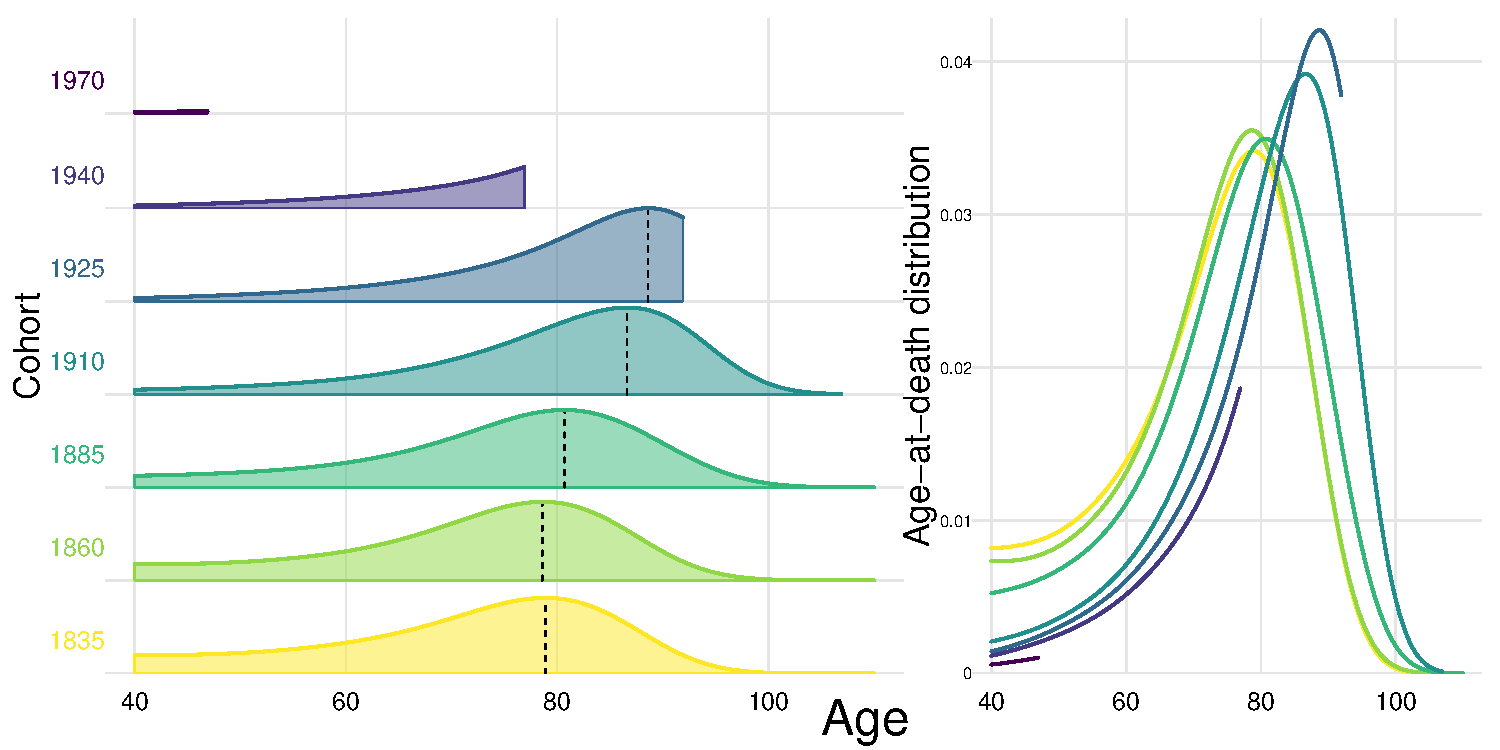
\includegraphics[scale=0.60]{./Figures/F1.pdf}
		\caption{Observed age-at-death distributions for Swedish females aged 40--110+ for selected cohorts between 1835--1970. Dashed black lines correspond to modal ages at death. Data have been smoothed for illustrative purposes. \\ \small \textit{Source}: Authors' elaborations on data from the \cite{HMD}.}\label{Fig:ADDcohort}	
	\end{center}
\end{figure}

Importantly, Figure \ref{Fig:ADDcohort} further motivates the development of a methodology that can leverage the features and the changes of age-at-death distributions with the purpose of modelling and forecasting human mortality. Clearly intelligible and demographically meaningful mortality developments readily emerge from this Figure. The left panel shows the increase of the modal age at death for the cohorts born after the 1860. In the right panel, the same distributions of the left panel are plotted over a common $y$-axis: decreasing age-at-death variability is evident for more recent cohorts.

Age-at-death distributions thus provide informative insights into mortality patterns and development of the population, and they further allow one to study the shifting and compression dynamics of mortality changes \cite[see, e.g.,][]{fries1980aging,kannisto2001mode,bongaarts2005long,janssen2019timing}. We therefore propose an approach to model and forecast adult cohort mortality that is based on age-at-death distributions. A relational model inspired by the seminal contribution of \cite{brass1971scale} serves our purposes well. Specifically, the combination of a reference distribution and its transformation over different cohorts allows us to simultaneously: (i) fit the observed data, and (ii) obtain estimates for the unobserved data, thereby completing the mortality experience of partially observed cohorts. In the following Section, we introduce our proposed methodology.  

\section{Methods \& Data}
\label{Sec:Methods}
\subsection{The C-STAD model}
\label{Subsec:C-STADmodel}
Suppose we have two adult age-at-death distributions defined on the age range $x \geq 40$. Specifically, let $f(x)$ be a "standard", or reference, distribution and $g(x)$ an observed distribution. Let $t(x;\bm{\theta})$ be a transformation function of the age axis and a vector of parameters $\bm{\theta}$ such that:
%
\begin{equation}\label{Eq:gxftx}
g(x) = f\left[t(x;\bm{\theta})\right]\,, 
\end{equation}  
%
i.e.~the distribution $g(x)$ is derived from a warping transformation of the age axis of $f(x)$. Specifically, the term ``warping'' originates in Functional Data Analysis \citep{ramsay2005FDA} and refers to the transformation of a time axis to achieve close alignment of functions. 

We propose a parsimonious yet flexible transformation function $t(x;\bm{\theta})$ that rigorously captures adult mortality developments across cohorts. Let $\bm{\theta}' = \left[s,b_{L},c_{L},d_{L},b_{U}\right]$ be a vector containing the model's parameters, where $s = M^{g} - M^{f}$ is the difference between the modal ages at death of the unimodal distributions $g(x)$ and $f(x)$. The proposed \emph{Cohort Segmented Transformation Age-at-death Distributions} (C-STAD) model can be written as: 
%
\begin{equation}\label{Eq:tx}
t(x;\bm{\theta}) = \left\{ \begin{array}{ll}
M^{f} + b_{L}\,\tilde{x} + c_{L}\,\tilde{x}^2 + d_{L}\,\tilde{x}^3 \quad & \mathrm{if} \; x \leq M^{g} \, \\
M^{f} + b_{U}\,\tilde{x} \quad & \mathrm{if} \; x > M^{g} \\
\end{array}
\right.
\end{equation} 
%
where $\tilde{x}=x - s - M^{f}$, and the subscripts $_L$ and $_U$ refer to the \textit{Lower} and \textit{Upper} parts of the segmented transformation (i.e.~before and after $M^{g}$), respectively. 

The warping function $t(x;\bm{\theta})$ takes the form of a segmented transformation model which breaks at the value of $M^{g}$. Below $M^{g}$, the transformation function is cubic, while it is linear above $M^{g}$. Although acting on $t(x;\bm{\theta})$, the model's parameters are directly related to the summary measures of the age-at-death distributions. Specifically, while $s$ captures the difference in modal ages between $g(x)$ and $f(x)$, $b_L$ and $b_U$ measure the change in variability before and after the modal ages of the two distributions. For the ages below $M^{g}$, $c_L$ and $d_L$ further measure differences in terms of asymmetry and heaviness of the left tail between $g(x)$ and $f(x)$, respectively. In terms of mathematical moments, the parameters $b_L$ and $b_U$ can be related to the variance of the distribution before and after the mode, while $c_L$ and $d_L$ relate to the skewness and kurtosis of the distribution. 

The modal age at death is a convenient location for segmenting the transformation in Eq.~\eqref{Eq:tx} for several reasons. In addition to being a central summary measure of the age-at-death distribution, the inspection of Figure~\ref{Fig:ADDcohort} (right panel) shows that mortality changes below the mode varied differently than above it. As such, it is useful to model and consider separately the two age ranges. Furthermore, the mode has been used to measure longevity in low-mortality countries \cite[see, e.g.,][]{kannisto2001mode,horiuchi2013modal}. Several studies have investigated changes in the variability of the age-at-death distribution above the mode from the period perspective \citep{kannisto2000measuring,kannisto2001mode,cheung2007increase,cheung2009dissecting,thatcher2010compression,ouellette2011changes}, because of the differences in mortality developments below and above the mode. Therefore, the segmentation of $t(x;\bm{\theta})$ at $M^{g}$ allows us to: (i) study changes in the age-at-death variability below and above the mode simultaneously, while considering different model specifications, and (ii) provide insights into age-at-death variability from the cohort perspective.

Figure~\ref{Fig:CSTADmodel} provides a graphical illustration of the C-STAD model. For ease of presentation, we start from the simpler case in which $b_L = b_U = 1$ and $c_L = d_L = 0$. Substitution of these parameters in Eq.~\eqref{Eq:tx} yields a unique transformation function $t(x;\bm{\theta})=x-s$, and a corresponding distribution $g_1(x) = f(x-s)$ via Eq.~\eqref{Eq:gxftx}. In the left panel of Fig.~\ref{Fig:CSTADmodel}, the standard distribution (grey line) is shifted to the right by an amount equal to $s$, and $g_1(x)$ (blue line) maintains the original shape of $f(x)$. The right panel shows the transformation function related to this plain shifting scenario. Note that a left-shift could be simply obtained with a negative value of $s$. 

\begin{figure}[t]
	\begin{center}
		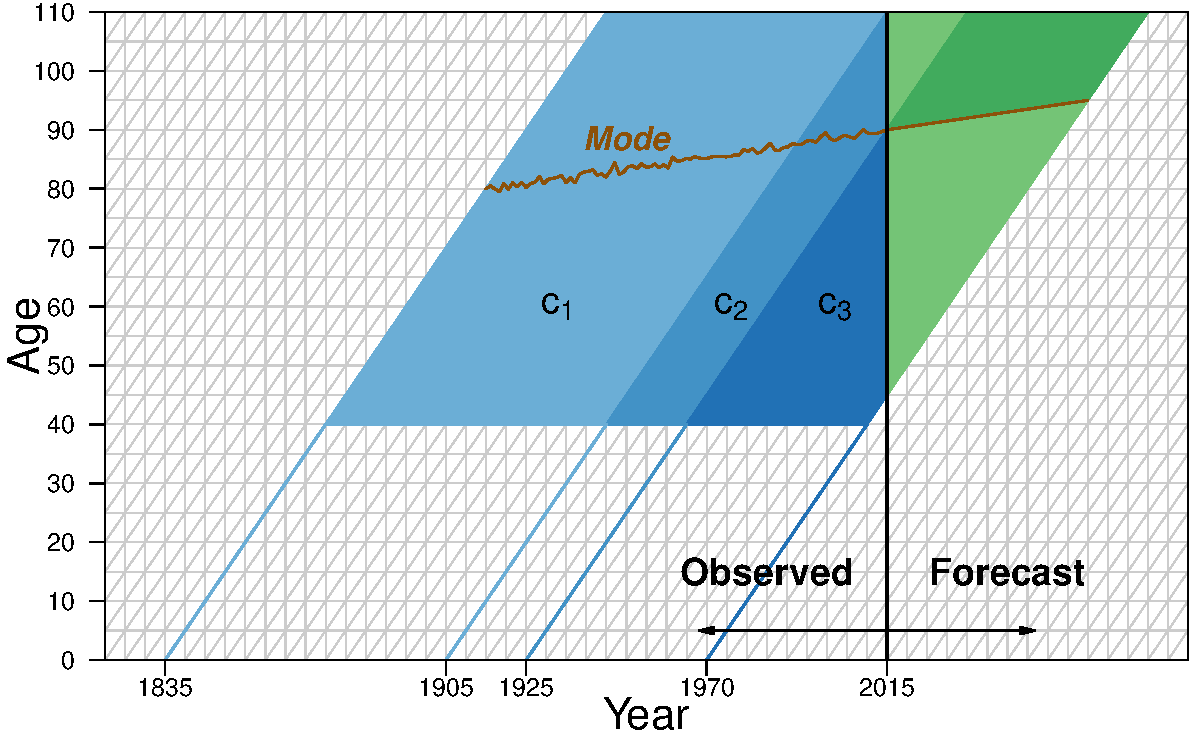
\includegraphics[scale=0.57]{./Figures/F2.pdf} 
		\caption{A schematic overview of the \emph{Cohort Segmented Transformation Age-at-death Distributions} model.\\
		\small \textit{Source}: Authors' own elaborations. \label{Fig:CSTADmodel}}    
	\end{center}
\end{figure}

Different parameters' values allow one to capture broader mortality developments than the shifting scenario described above. While $b_L$ and $b_U$ modify the variability of the distribution $g_2(x)=f\left[t(x;\bm{\theta})\right]$ (orange line, left panel) w.r.t.~$f(x)$ before and after the modal age at death, $c_L$ and $d_L$ affect the asymmetry and heaviness of the left tail of $g_2(x)$ as compared to $f(x)$. In the example shown in Fig.~\ref{Fig:CSTADmodel}, $b_L > 1$ reduces the variability of $g_2(x)$ before $M^g$ w.r.t.~$f(x)$, while $b_U < 1$ increases the variability of $g_2(x)$ after $M^g$ w.r.t.~$f(x)$. The effects of $c_L$ and $d_L$ are difficult to discern from the left panel. However, the right panel shows the warping transformation $t(x;\bm{\theta})$ applied to $f(x)$ to derive $g_2(x)$; the transformation (orange line) is composed of a cubic function (due to non-zero values of $c_L$ and $d_L$) before the cut-off point $M^g$, and a linear function above $M^g$.

\subsection{Data}
\label{Subsec:Data}
For illustrative purposes we present outcomes from the proposed model on adult cohort mortality for females in two high-longevity countries, namely Sweden and Denmark. Long-term series of high quality data are available for both countries, even at very old ages \citep{vaupel1994longer,wilmoth1996extreme,AndreevBookDanemark}, and the two countries display different mortality developments. We therefore test the goodness-of-fit and forecast accuracy of our model with respect to different mortality trajectories \citep{christensen2010divergent}. The data are derived from the \citeauthor{HMD} (HMD, \citeyear{HMD}), which provides free access to detailed, consistent and high quality historical mortality data for 41 different areas and countries \citep{barbieri2015data}.

Our interest in this article is restricted to the senescent component of mortality, hence we start our analyses from age 40. We therefore cover the age range that is of greater interest for pension and insurance funds. Specifically, we work with two $m \times n$ matrices $\bm{D} = (d_{x,c})$ and $\bm{E} = (e_{x,c})$, defined for ages $\bm{x}'=\left[40,\dots,110+\right]$ and cohorts $\bm{c}'=\left[1835,\dots,1970\right]$. Figure~\ref{Fig:Lexis} offers a schematic overview of the data structure by means of two Lexis diagrams: the first (left panel) shows the conventional age-period structure, while the second (right panel) illustrates the age-cohort perspective that we adopt in this paper. On the one hand, we select 1835 as starting cohort of analysis for both populations because it is the first cohort with observed data at all ages in Denmark, and to compare the results for the two countries using the same fitting period. On the other hand, 1970 is the final cohort because it contains enough observed data points in both countries (seven in Sweden, six in Denmark) to accurately estimate the three parameters of the lower part of the transformation function in Eq.~\eqref{Eq:tx} (i.e.~$b_L$, $c_L$ and $d_L$, cf.~Subsection \ref{Subsec:EstimForeC-STAD}). 

\begin{figure}[t]
	\begin{center}
		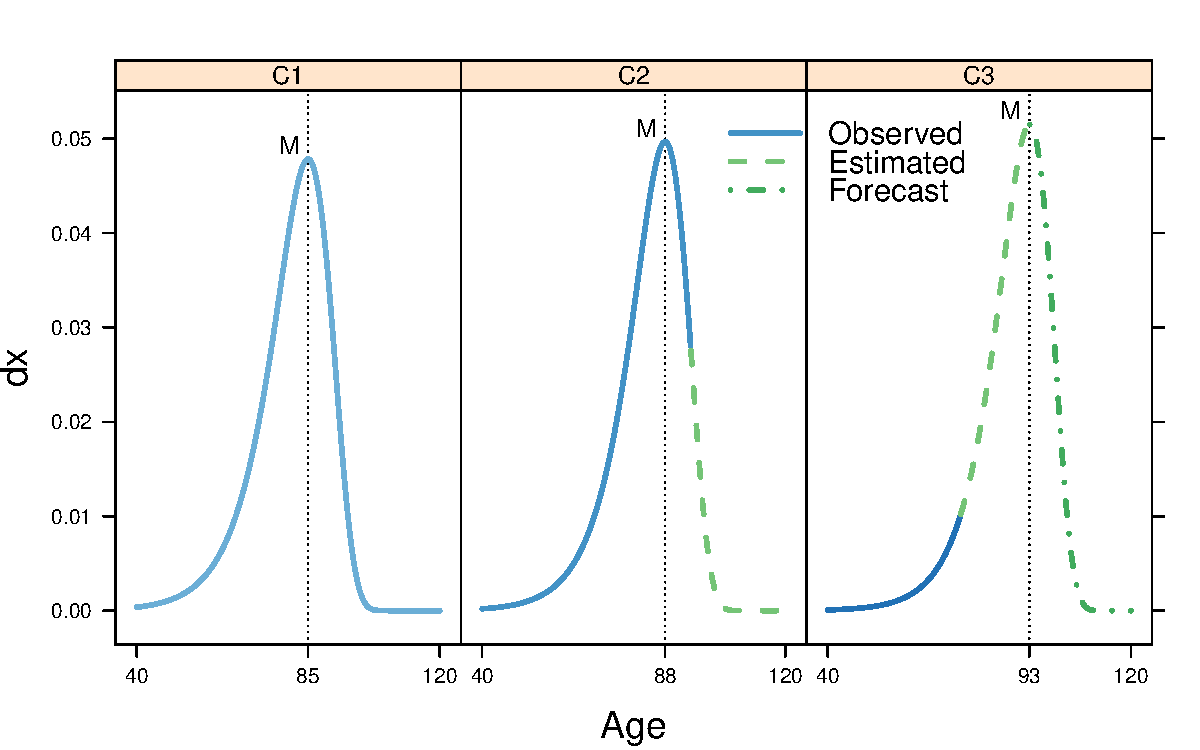
\includegraphics[scale=0.7]{./Figures/F3.pdf} 
		\caption{Conventional age-period (left panel) and age-cohort (right panel) Lexis diagrams illustrating the data structure and the division of cohorts into three groups. Here we assume that: (i) 2015 is the most recent year of data collection, (ii) $\breve{c}=1905$, and (iii) $\tilde{c}=1925$. The three groups are then $\bm{c}'_1=\left[1835,\dots,1905\right]$, $\bm{c}'_2=\left[1906, \dots, 1925\right]$ and $\bm{c}'_3=\left[1926, \dots, 1970\right]$. The two colours in the forecast years correspond to different parameters' derivations (cf.~Subsection \ref{Subsec:EstimForeC-STAD}): estimation with incomplete data (light green) and forecasting (dark green). \\
		\small \textit{Source}: Authors' own elaborations. \label{Fig:Lexis}}    
	\end{center}
\end{figure}

%\newpage

Estimation and forecasting of the C-STAD parameters (Subsection \ref{Subsec:EstimForeC-STAD}) is performed on three different groups of cohorts:
\begin{equation}\label{eq:CohortDiv}
\bm{c}' = \left[ \, \tikzmark{lowerC1}1835 \, , \dots , \, \breve{c}\tikzmark{upperC1} \, , \, \tikzmark{lowerC2}\breve{c}+1 \, , \dots, \, \tilde{c}\tikzmark{upperC2} \, , \, \tikzmark{lowerC3}\tilde{c} + 1 \, , \dots, \, 1970\tikzmark{upperC3} \, \right] \, .
\end{equation}	

\begin{tikzpicture}[overlay, remember picture,decoration={brace,amplitude=5pt}]
\draw[decorate,thick] (upperC1.south) -- (lowerC1.south)
node [midway,below=5pt] {$\bm{c}_1$};
\draw[decorate,thick] (upperC2.south) -- (lowerC2.south)
node [midway,below=5pt] {$\bm{c}_2$};
\draw[decorate,thick] (upperC3.south) -- (lowerC3.south)
node [midway,below=5pt] {$\bm{c}_3$};
\end{tikzpicture}

Therefore the data are partitioned as follows:
\begin{equation}\label{eq:DataDiv}
\bm{D} = \left[ \bm{D}_{1} : \bm{D}_{2} : \bm{D}_{3}\right] \qquad \bm{E} = \left[ \bm{E}_{1} : \bm{E}_{2} : \bm{E}_{3}\right] \, .
\end{equation}
The first group, denoted by $\bm{c}_1$, contains the fully observed cohorts $1835,\ldots,\breve{c}$, where $\breve{c}$ corresponds to the last cohort for which all data have been observed. As such, $\bm{D}_{1}$ and $\bm{E}_{1}$ have been observed at all ages $x$ for all cohorts in $\bm{c}_1$. The second group, denoted by $\bm{c}_2$, is composed by cohorts $\breve{c}+1, \ldots, \tilde{c}$, where $\tilde{c}$ corresponds to the last cohort for which two age-groups above the adult modal age at death have been observed. In other words, $\bm{D}_{2}$ and $\bm{E}_{2}$ are incomplete, i.e.~data are not available for higher ages and more recent cohorts. However this group of cohorts is selected such that associated $d_{x,c}$ and $e_{x,c}$ have been observed for at least two data points above the modal age $x=M$ for all cohorts in $\bm{c}_2$. The choice of having two age groups above $M$ is imposed by the estimation of the parameter above the mode (cf.~Subsection~\ref{Subsec:EstimForeC-STAD}). Finally, the third group $\bm{c}_3$ is composed of the remaining cohorts $\tilde{c}+1, \ldots, 1970$, in which data are only partially available and modal age at death is not observed. An illustration of the divisions of cohorts into the three groups is provided in Figure~\ref{Fig:Lexis}. Figure \ref{Fig:DxExample} shows an example of the observed and missing data for three age-at-death distributions belonging to the different groups of cohorts. 

\begin{figure}[t]
	\begin{center}
		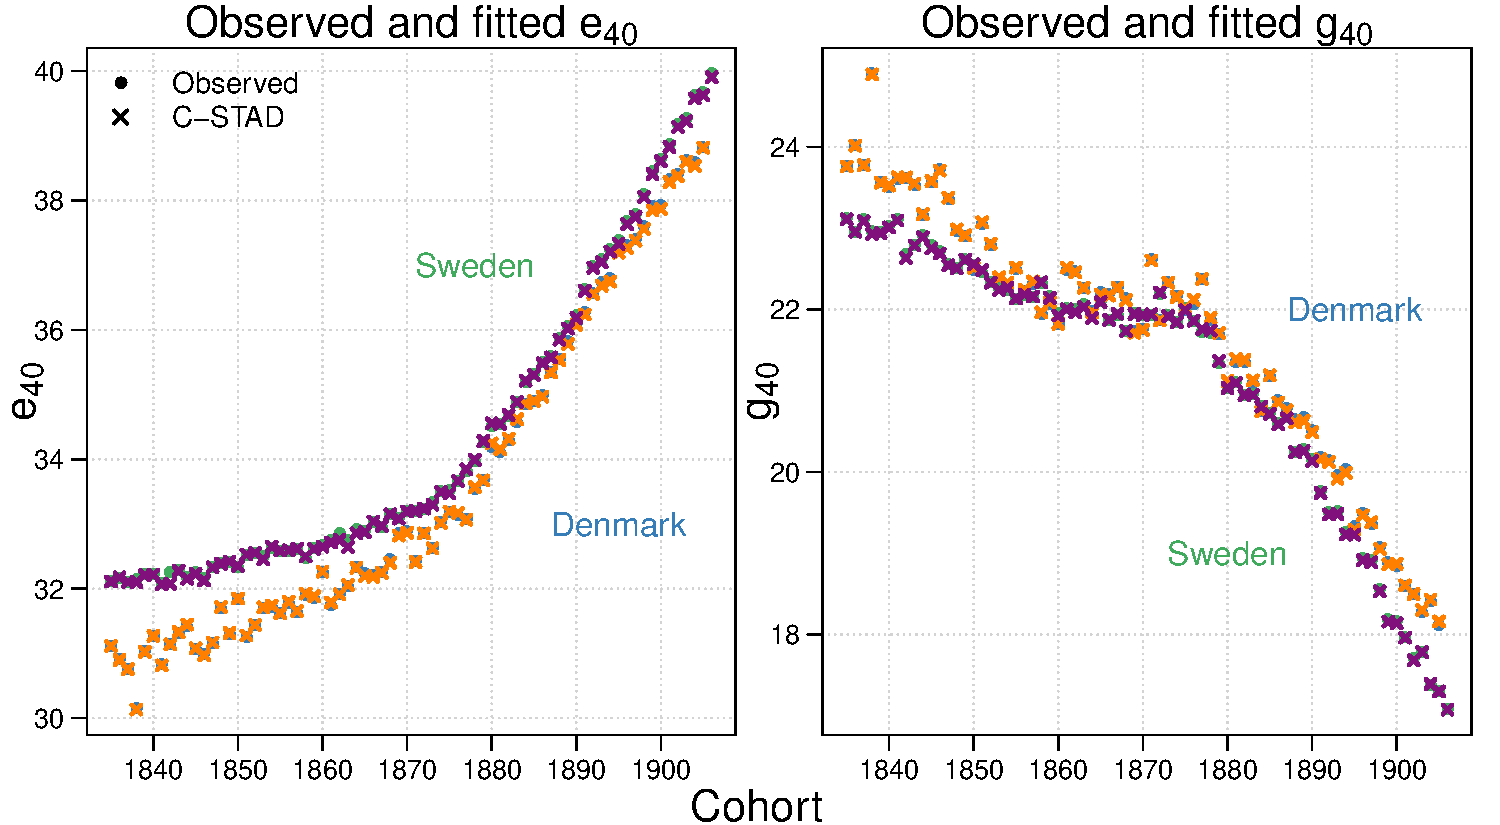
\includegraphics[scale=0.7]{./Figures/F4.pdf} 
		\caption{Example of observed, estimated and forecast data for three age-at-death distributions belonging to the groups of cohorts $\bm{c}_1$, $\bm{c}_2$ and $\bm{c}_3$.\\
		\small \textit{Source}: Authors' own elaborations.\label{Fig:DxExample} }    
	\end{center}
\end{figure}

\subsection{The standard distribution}
\label{Subsec:Standard}
The first step in the estimation of the C-STAD model is the derivation of the standard distribution $f(x)$. The C-STAD can be interpreted as a relational model \citep{brass1971scale}, hence it is desirable to include the representative features of the observed data for all cohorts in the computation of $f(x)$. Meanwhile, we also wish to remove the small random fluctuations that characterize the mortality pattern of age-at-death distributions. To achieve both goals at the same time, we derive the age-at-death distribution for each cohort 1835--1970 by a two-dimensional (2D) $P$-splines smoothing approach to cohort mortality \citep{eilers1996flexible, currie2004smoothing}. Specifically, we assume that observed death counts $d_{x,c}$ at given age $x$ and cohort $c$ are realizations of the random variable $D_{x,c}$ which follows a Poisson distribution \citep{brillinger1986biometrics}:
%
\begin{equation}\label{Eq:Poisson}
D_{x,c} \sim \mathcal{P}(e_{x,c} \; \mu_{x,c}) \, ,
\end{equation}
%
where exposures-to-risk $e_{x,c}$ are given and $\mu_{x,c}$ denote the hazard or force of mortality \cite[such as in, for example,][]{brouhns2002poisson}. We smooth observed death counts using a tensor product of $B$-spline bases over ages and cohorts, and exposures as an offset. To account for incomplete cohorts and still preserve the rectangular structure in the data, we include regression weights $\bm{W} = (w_{x,c})$ whose elements are equal to one if the corresponding death counts $d_{x,c}$ and exposures $e_{x,c}$ have been observed, and zero otherwise. Smoothing parameters over ages and cohorts are chosen by Bayesian Information Criterion minimization. The \texttt{R} package \texttt{MortalitySmooth} \citep{camarda2012mortalitysmooth} provides a direct implementation of this procedure. 

The estimated smooth mortality surface allows us to derive smooth (partial) distributions. To compute the standard, we first employ a landmark registration procedure, a technique often used in Functional Data Analysis with the aim of aligning important features, or landmarks, of the curves analysed \citep{ramsay2005FDA}. For age-at-death distributions, the modal age at death is an obvious landmark. As such, we align the distributions so that their modal ages are equal to the mode of the first observed distribution (the 1835 cohort), maintaining their variability unchanged. In practice, the alignment is achieved by a plain shifting transformation of the observed distributions, which preserves all their features except the modal age-at-death. 

Having aligned the observed distributions to a common modal age, we derive the standard $f(x)$ as the mean of the aligned distributions. Figure \ref{Fig:Alignment} in Appendix \ref{Appendix:AdditResults} illustrates the alignment procedure and the derivation of the standard distribution for the Swedish female population analysed in our article. This landmark registration procedure enhances the representativeness of $f(x)$ while improving the goodness-of fit of the model \cite[for additional details, see][]{basellini2019modelling}. Importantly, it should be noted that for cohorts in $\bm{c}_2$ and $\bm{c}_3$, we only use the part of the aligned distribution corresponding  to the observed data (i.e.~where regression weights are not zero). 

Finally, we express the standard $f(x)$ as a linear combination of equally spaced $B$-spline bases $\bm{B}(x)$ over ages $x$ and coefficients $\bm{\beta}_{f}$ specific to the standard:
%
\begin{equation}\label{Eq:standPsplines}
f(x) = \exp\left[ \bm{B}(x) \, \bm{\beta}_{f} \right] \, .
\end{equation}
In this last step, we chose a generous number of $B$-splines with a small penalty term. This whole procedure allows us to preserve all important features in the standard distribution (embodied in $\bm{\beta}_{f}$) after having removed unnecessary random fluctuations from the original data. In addition, the smoothing approach further allows us to evaluate mortality at any finer scale of the age axis, practically at a continuous level.


\subsection{Estimation and forecast of the C-STAD parameters}
\label{Subsec:EstimForeC-STAD}
Given the estimated standard distribution, we can derive the C-STAD parameters $\bm{\theta}'=\left[s,b_{L},c_{L},d_{L},b_{U}\right]$ for each cohort in 1835--1970. As anticipated in Subsection \ref{Subsec:Data}, we use three different approaches to estimate $\bm{\theta}$, depending on the data available for each cohort; we thus divide cohorts into three groups, as shown in Figure \ref{Fig:Lexis}. 

For the first group of fully observed cohorts $\bm{c}_1$, we start by estimating the parameters vector $\bm{s}$. To properly capture cohort-specific mortality fluctuations, we employ a one-dimensional $P$-spline approach, i.e.~we smooth mortality for each cohort independently, numerically compute the corresponding density and extract the modal ages at death for each cohort \citep[for a similar approach in a period perspective, see][]{ouellette2011changes}. From the modal ages we estimate the parameter $\hat{\bm{s}}=\left(\hat{s}_{c}=M_{c} - M_f\right)$ over cohorts in $\bm{c}_1$, where $M_f$ denotes the mode of the standard distribution, which by construction corresponds to the modal age at death for the cohort born in 1835. \par

Having derived an estimate of the shifting parameter $\hat{\bm{s}}$, we can estimate the remaining parameters $\bm{\alpha}'=\left[b_{L},c_{L},d_{L},b_{U}\right]$. We take advantage of the Poisson assumption in Eq.~(\ref{Eq:Poisson}) and maximise the following log-likelihood function:
%
\begin{equation}\label{Eq:loglikeC1}
\ln\mathcal{L}_{\bm{\alpha}}\left(\bm{\alpha}\,|\,d_{x,c} , e_{x,c} , w_{x,c} , \hat{s}_{c}, \bm{\beta}_{f}
\right) \propto \sum_{x} w_{x,c} \left[  d_{x,c} \,
\ln \left( \mu^{\texttt{C-STAD}}_{x,c}  \right) - e_{x,c}
\, \mu^{\texttt{C-STAD}}_{x,c} \right] 
\end{equation}
%
for each cohort in $\bm{c}'_1 = \left[1835,\dots,\breve{c}\right]$, where regression weights $w_{x,c}$ are zero in the case of unobserved data at the highest ages, and $\mu^{\texttt{C-STAD}}_{x,c}$ denotes the estimated hazard of the C-STAD model. In words, the optimization procedure looks for a combination of parameters $\hat{\bm{\alpha}}$ that produces, for each cohort, an age-at-death distribution whose corresponding hazard maximises the log-likelihood in Eq.~(\ref{Eq:loglikeC1}). The associated age-at-death distribution $\hat{g}_{c}(x)$ can be written as follows:
\begin{equation}\label{eq:gBspl}
\hat{g}_{c}(x) = \exp\left[ B(x_{t}) \bm{\beta}_{f} \right] \qquad \mbox{where} \quad x_{t} = t(x; \hat{s}_{c},\hat{\bm{\alpha}}) \, .
\end{equation}
The hazard $\hat{\mu}_c(x)$ corresponding to $\hat{g}_{c}(x)$ is computed using standard life-table and survival analysis formulas:
\begin{equation}\label{Eq:HazardCSTAD}
\hat{\mu}_c(x) = \frac{\hat{g}_c(x)}{\hat{\ell}_c(x)} = \frac{\hat{g}_c(x)}{\int_{x}^{\infty} \hat{g}_c(t)\,dt} \, ,
\end{equation}
where $\hat{\ell}_c(x)$ denotes the life-table probability of surviving to age $x$ \cite[i.e.~the survival function,][]{preston2001demogr,klein2003survival}, which can be computed numerically from the smooth distribution $\hat{g}_{c}(x)$, evaluated at an extremely fine level.

For the second group of partially observed cohorts $\bm{c}_2$, we start again from the shifting parameter $\bm{s}$. We use the same estimation approach used in $\bm{c}_1$: data are available until the ages above the mode, therefore the smoothing approach produces an estimate of $M_c$ and $\hat{\bm{s}}$ over cohorts in $\bm{c}_2$. With respect to the remaining parameters, we also follow the same approach: we maximize Eq.~\eqref{Eq:loglikeC1} for each cohort in $\bm{c}'_2=\left[\breve{c}+1,\ldots,\tilde{c}\right]$, the only difference being that zero regression weights correspond to the missing data above the mode of the partially observed cohorts. It should be noted here that the unobserved data only influence the estimation of $b_U$, as complete data are observed below the mode for all cohorts in this group. 

For the third group of partially observed cohorts $\bm{c}_3$, we employ a mixture of forecasting and estimation to determine the C-STAD parameters. The lack of data above the modal age at death makes it impossible to estimate the parameter $\bm{s}$ and compute the log-likelihood in Eq.~\eqref{Eq:loglikeC1}. Hence, we start from the time-series of the estimated parameters $\hat{\bm{s}}$ and $\hat{\bm{b}}_U$ over cohorts in $\bm{c}_1$ and $\bm{c}_2$ to compute their forecasts for cohorts $\bm{c}_3$. 

From a theoretical perspective, these two parameters are related by the fact that only mortality changes occurring above the mode can modify its value \cite[cf.~Appendix B in][]{canudas2010three}. Correlation analyses for the two countries under study confirm the strong relation between the two series (Pearson correlation of 0.96 and 0.90 for the time-series in first differences for Sweden and Denmark, respectively). As such, we specify a vector autoregressive (VAR) model of order one with a constant for the two (differenced) parameters, and we forecast their values for all cohorts $\bm{c}_3$. The \texttt{R} package \texttt{vars} allows us to perform model selection and estimation \citep{pfaff2008analysis,pfaff2008var}.

Then, we take the forecast values of $\hat{\bm{s}}$ and $\hat{\bm{b}}_U$ as given, and we estimate the remaining parameters $\breve{\bm{\alpha}}'=\left[b_{L},c_{L},d_{L}\right]$ by maximizing the log-likelihood:
%
\begin{equation}\label{Eq:loglikeC3}
%\begin{aligned}
\ln\mathcal{L}_{\breve{\bm{\alpha}}}\left(\breve{\bm{\alpha}}\,|\,d_{x,c} , e_{x,c} , w_{x,c} , \hat{s}_{c}, \hat{b}_{U_{c}} , \bm{\beta}_{f} \right) \propto  \sum_{x} w_{x,c} \, \left[  d_{x,c} \,
\ln \left( \mu^{\texttt{C-STAD}}_{x,c}  \right) - e_{x,c}
\, \mu^{\texttt{C-STAD}}_{x,c} \right] 
%\end{aligned}
\end{equation}
%
for each cohort in $\bm{c}'_3=\left[\tilde{c}+1,\ldots,1970\right]$. In contrast to the estimation procedure in $\bm{c}_2$, here the unobserved data influence the estimation of the parameters associated to the ages below the modal age at death. 

The estimate $\hat{\bm{\theta}}$ for each cohort in 1835--1970 allows us to derive a complete set of age-specific mortality measures, i.e.~we can complete the mortality experience for the partially observed cohorts of our analysis. In order to derive the C-STAD confidence intervals (CI)\footnote{to avoid confusion, we use the general term CI for all cohorts analysed, even when intervals are constructed from the mixture of forecast and estimated parameters (i.e.~cohorts $\bm{c}_3$).}, we employ a bootstrapping procedure \citep{efron1994introduction}. As suggested by \cite{keilman2006prediction}, we consider the uncertainty related to: (i) the estimated parameters, and (ii) the forecast values of $\bm{s}$ and $\bm{b}_U$. The first source of uncertainty is accounted for by generating bootstrap death counts from the C-STAD deviance residuals \cite[as in, for example,][]{koissi2006evaluating,renshaw2008simulation,ouellette2012regional}. Appendix \ref{Appendix:ResidualDeath} provides more details on the computation of deviance residuals and bootstrap death counts. The second source of uncertainty is considered by simulating future values of the VAR model. We employ 40 different matrices of bootstrap death counts, and for each of these, we refit the C-STAD model and simulate 40 future values of $\bm{s}$ and $\bm{b}_U$. From the 1600 resulting simulations, we take the lowest and highest deciles to construct 80\% pointwise confidence intervals.

Finally, routines developed to fit and forecast the C-STAD model were implemented in \texttt{R} \citep{Rcite} and are publicly available, and all the results presented in the following Section are fully reproducible at \url{https://github.com/ubasellini/C-STAD} [this GitHub repository will be made public upon eventual acceptance of the manuscript]. 

\section{Results}
\label{Sec:Results}

\subsection{Out-of-sample validation of the C-STAD model}
\label{Subsec:Out-of-sample}
Before estimating the proposed C-STAD model to complete partially observed cohorts, we first assess the accuracy of the C-STAD model by performing six predictive out-of-sample validation exercises on Swedish and Danish adult females. We compare the forecast life expectancy at age 40 ($e_{40}$) and the Gini coefficient at age 40 ($G_{40}$) with the observed out-of-sample values. Both measures of longevity (the former) and lifespan inequality (the latter) are useful to evaluate the accuracy of mortality forecasts \citep{bohk2017lifespan}. 

Formally, the Gini coefficient at age 40 is defined as:
%
\begin{equation}\label{Eq:GINI}
G_{40} = 1 - \frac{1}{e_{40}\,\left(\ell_{40}\right)^2} \int_{40}^{\omega} \left[\ell(x)\right]^2 dx \, ,
\end{equation}
%
where $\ell_{40}$ is the life-table radix, which we set equal to one without loss of generality, and $\omega$ is the highest age attained in the population \citep{hanada1983formula,shkolnikov2003gini}.

Originally proposed to measure income or wealth inequality \citep{gini1912variabilita,gini1914sulla}, the Gini coefficient is today one of the most common statistical indices employed for measuring concentration in the distribution of a positive random variable. In recent years, the coefficient has been used to measure lifespan inequality within and between populations \cite[see, e.g.,][]{shkolnikov2003gini,smits2009length,van2013perturbation,gigliarano2017longevity} and to evaluate mortality forecasts \citep{diaz2018mortality,basellini2019modelling}. The coefficient takes values between 0 and 1, which correspond to the limit cases of perfect equality and perfect inequality, respectively. For an age-at-death distribution, Gini is equal to zero if all individuals die at the same age, and equal to 1 if all people die at age 0 and one individual dies at a positive age \citep{shkolnikov2003gini}. In this article, we compute $G_{40}$ in Eq.~\eqref{Eq:GINI} with the approximation formula proposed by \cite{shkolnikov2003gini}, and we multiply $G_{40}$ by 100 in order to have a comparable magnitude with $e_{40}$.

Specifically, we pretend that the last year of collected data is $2015 - h$, where $h=10$, 15, 20, 25, 30 and 35 years. We then fit the C-STAD model to the fully observed cohorts $\bm{c}'_1=\left[1835,\dots,1905-h\right]$, and we forecast mortality $h$ years ahead. If the modal age is always observed for the cohorts to be completed, the exercise is restricted to the group $\bm{c}_{2}$. Otherwise, the group $\bm{c}_{3}$ is considered too. 

An explicative example of the validation procedure is useful to clarify the out-of-sample exercises. Let us consider $h=10$: then, the last year of fully observed data is 2005. We fit the C-STAD to the fully observed cohorts $\bm{c}'_1=\left[1835,\dots,1895\right]$, and we forecast 10-year ahead. By doing so, we complete the mortality experience of the partially observed cohorts $1896,\ldots,1905$, and for each of these, we compute and compare the estimated $e_{40}$ and $G_{40}$ with their observed values. 

It is worth mentioning at this point that, for the lower values of $h$, forecasting is achieved simply by fitting the C-STAD on the partially observed cohorts $\bm{c}_2$. In the explicative example above, where the last data available occurred in 2005, the cohort 1896, for instance, has been observed at all ages except 110. We thus take advantage of the nature of cohort data and consider all possible observations to complete the mortality experience of this partial cohort.  Conversely, for higher values of $h$, forecasting is achieved by considering also the cohorts $\bm{c}_3$, which require the combination of forecasting and estimation of the C-STAD parameters. 

In addition to the C-STAD, we perform the same out-of-sample exercises with the 2D $P$-splines approach of \cite{currie2004smoothing}. This is the only model that, to our knowledge, has been employed to forecast cohort mortality from a cohort perspective \citep{cmi2007stochastic} and can be implemented in the \texttt{R} software after data manipulation \cite[in the \texttt{MortalitySmooth} package,][]{camarda2012mortalitysmooth}. 

Furthermore, we compare our results with the standard procedure of: (i) forecasting mortality in an age-period fashion, and (ii) extracting cohort patterns from the diagonals of the age-period mortality surface. For these comparisons, we employ two models on the age-period perspective: the benchmark Lee-Carter (LC) model \citep{lee1992modeling}, and the age-period-cohort (APC) model employed by \cite{currie2012forecasting,currie2019constraints}. The LC model was fitted using the \texttt{demography} package \citep{demogRpackage}, while the APC model with the \texttt{StMoMo} package \citep{villegas2018stmomo}. For consistency, in each exercise we select the shortest fitting period that includes all the cohorts needed to assess the forecasts from the age-period surface. Fitting periods for the six exercises are 1936--2005, 1931--2000, 1926--1995, 1921--1990, 1916--1985 and 1911--1980: the starting year is computed by adding 40 (the starting age of the analysis) to the first forecast cohort, while the last year is given by $2015 - h$. It should be noted that the fitting age-period surface for these exercises was derived from the original age-cohort data, to exclude potential bias related to differences in the computation of period vs.~cohort mortality rates \cite[see][pp.~29--33]{wilmoth2019protocol}. 

%We do not consider other methodologies, such as the \cite{lee1992modeling} model and its variants, because cohort forecasts with these approaches are derived from period ones, and the comparison would not be objective (for example, forecast values depend on the length of the fitting period, whose choice would be subjective and not comparable in such exercise).  

Table \ref{Table:RMSE} presents the results of our analysis. The first and second columns contain the cohorts used for fitting and forecasting the C-STAD and 2D $P$-splines models, respectively. The third column contains the forecast horizon of the out-of-sample exercise, while the fourth column indicates the measure analysed ($e_{40}$ and $G_{40}$). Results are shown in the last eight columns. We assess the accuracy of the point forecasts by computing the root mean square error (RMSE):
%
\begin{equation}\label{Eq:RMSE}
\mathrm{RMSE}=\sqrt{\frac{1}{h} \sum_{c=1}^{h} \left(\hat{y}_c-y_c\right)^2} \, , \notag
\end{equation} 
%
where $h$ is the forecasting horizon, and $\hat{y}_c$ and $y_c$ are the forecast and observed out-of-sample values of either $e_{40}$ or $G_{40}$. 

The table shows that the C-STAD forecasts are accurate in completing the mortality experience of partially observed cohorts. The RMSE values of both $e_{40}$ and $G_{40}$  are low across the six exercises, and they do not increase significantly with the forecasting horizon. Additionally, C-STAD forecasts are more accurate than those of the 2D $P$-spline model. Both the C-STAD and the 2D $P$-spline models significantly outperform the standard LC age-period approach. Furthermore, both models are more accurate than the APC model based on the age-period perspective, whose consideration of the additional cohort parameter improves the forecasting performance compared to the LC model. Employing different fitting periods in the age-period exercises, such as starting the analysis from the same year (for example, 1911) in all cases, would result in even greater RMSE for the LC forecasts for the shorter horizon exercises. Very similar results are obtained by employing different prediction accuracy measures, such as the MAPE and MAE (see Appendix \ref{Appendix:AdditResults}).

\begin{landscape}
	% TABLE RMSE: 10, 20, 30 YEARS
	\begin{table}[t]
		\small
		\centering
		\begin{tabular}{cccccccc|cccc}
			\toprule
			& & & &   \multicolumn{4}{c|}{\textbf{Sweden}}    & \multicolumn{4}{c}{\textbf{Denmark}} \\
			
			\cmidrule{5-12}	
			
			\thead{Fitting \\ cohorts}  & \thead{Forecast \\ cohorts} & Horizon &  Measure  &  C-STAD   & \thead{2D \\ $P$-spline} & \thead{LC \\ (period)} & \thead{APC \\ (period)} &  C-STAD   & \thead{2D \\ $P$-spline}  & \thead{LC \\ (period)} &  \thead{APC \\ (period)}  \\ 
			\midrule	
			%%%% FIRST EXERCISE	
			\rowcolor{my-white} 
			\multicolumn{1}{c}{\cellcolor{my-white}}   &
			\multicolumn{1}{c}{\cellcolor{my-white}}   & \multicolumn{1}{c}{\cellcolor{my-white}}               & \multicolumn{1}{c|}{\cellcolor{my-white}$e_{40}$} & 0.08  & \textbf{0.08} & 0.22 & 0.13 & 0.08 &  0.08   & 0.41 & \textbf{0.06}  \\
			\rowcolor{my-white} 
			\multicolumn{1}{c}{\multirow{-2}{*}{\cellcolor{my-white}1835--1895}}  &  \multicolumn{1}{c}{\multirow{-2}{*}{\cellcolor{my-white}1896--1905}}  & 
			\multicolumn{1}{c}{\multirow{-2}{*}{\cellcolor{my-white}10y}}& \multicolumn{1}{c|}{\cellcolor{my-white}$G_{40}$} & \textbf{0.09} &   0.10 & 0.32 & 0.24 & \textbf{0.08} &  0.08 & 0.38 & 0.11 \\
			
			%%%% SECOND EXERCISE	
			\hhline{|------------|}
			\rowcolor{my-grey} 
			\multicolumn{1}{c}{\cellcolor{my-grey}}  & \multicolumn{1}{c}{\cellcolor{my-grey}}             &
			\multicolumn{1}{c}{\cellcolor{my-grey}}  & \multicolumn{1}{c|}{\cellcolor{my-grey}$e_{40}$} & \textbf{0.07} &  0.09 & 0.26 & 0.10 & \textbf{0.07} & 0.08 & 0.41 & 0.08 \\
			\rowcolor{my-grey}       \multicolumn{1}{c}{\multirow{-2}{*}{\cellcolor{my-grey}1835--1890}} &      \multicolumn{1}{c}{\multirow{-2}{*}{\cellcolor{my-grey}1891--1905}}               &
			\multicolumn{1}{c}{\multirow{-2}{*}{\cellcolor{my-grey}15y}}               & \multicolumn{1}{c|}{\cellcolor{my-grey}$G_{40}$} & \textbf{0.08} &  0.10 & 0.40 & 0.23 & \textbf{0.07} & 0.12  & 0.44 & 0.21    \\ 
			
			%%%% THIRD EXERCISE
			\hhline{|------------|}
			\rowcolor{my-white} 
			\multicolumn{1}{c}{\cellcolor{my-white}}   &
			\multicolumn{1}{c}{\cellcolor{my-white}}   &    \multicolumn{1}{c}{\cellcolor{my-white}}                & \multicolumn{1}{c|}{\cellcolor{my-white}$e_{40}$} &  \textbf{0.05} & 0.08 & 0.35 & 0.10 & \textbf{0.06} & 0.08 & 0.44 & 0.09 \\
			\rowcolor{my-white}            
			\multicolumn{1}{c}{\multirow{-2}{*}{\cellcolor{my-white}1835--1885}}           &
			\multicolumn{1}{c}{\multirow{-2}{*}{\cellcolor{my-white}1886--1905}}               &
			\multicolumn{1}{c}{\multirow{-2}{*}{\cellcolor{my-white}20y}}               & \multicolumn{1}{c|}{\cellcolor{my-white}$G_{40}$} & \textbf{0.09} & 0.11 & 0.53 & 0.28 & \textbf{0.06} & 0.12 & 0.45 & 0.25  \\
			
			%%%% FOURTH EXERCISE	
			\hhline{|------------|}
			\rowcolor{my-grey} 
			\multicolumn{1}{c}{\cellcolor{my-grey}}   &
			\multicolumn{1}{c}{\cellcolor{my-grey}}   & \multicolumn{1}{c}{\cellcolor{my-grey}}  & \multicolumn{1}{c|}{\cellcolor{my-grey}$e_{40}$} & \textbf{0.04} & 0.08 & 0.41 & 0.12  & \textbf{0.03} &  0.08  & 0.47  & 0.12 \\
			\rowcolor{my-grey} 
			\multicolumn{1}{c}{\multirow{-2}{*}{\cellcolor{my-grey}1835--1880}}   &  \multicolumn{1}{c}{\multirow{-2}{*}{\cellcolor{my-grey}1881--1905}}  & 
			\multicolumn{1}{c}{\multirow{-2}{*}{\cellcolor{my-grey}25y}}  & \multicolumn{1}{c|}{\cellcolor{my-grey}$G_{40}$} & \textbf{0.10} & 0.11 & 0.57 & 0.31 & \textbf{0.11} & 0.14  & 0.47  & 0.24  \\
			
			%%%% FIFTH EXERCISE
			\hhline{|------------|}
			\rowcolor{my-white} 
			\multicolumn{1}{c}{\cellcolor{my-white}}             &
			\multicolumn{1}{c}{\cellcolor{my-white}}             & \multicolumn{1}{c}{\cellcolor{my-white}}             & \multicolumn{1}{c|}{\cellcolor{my-white}$e_{40}$} &   \textbf{0.06} & 0.09 & 0.48 & 0.15 &  \textbf{0.03} &  0.11 & 0.52 & 0.16 \\
			\rowcolor{my-white} 
			\multicolumn{1}{c}{\multirow{-2}{*}{\cellcolor{my-white}1835--1875}} &      \multicolumn{1}{c}{\multirow{-2}{*}{\cellcolor{my-white}1876--1905}}               &
			\multicolumn{1}{c}{\multirow{-2}{*}{\cellcolor{my-white}30y}}               & \multicolumn{1}{c|}{\cellcolor{my-white}$G_{40}$} & \textbf{0.10} &  0.14 & 0.63 & 0.36 & \textbf{0.11} & 0.19   & 0.52 & 0.27   \\
			
			%%%% SIXTH EXERCISE
			\hhline{|------------|}
			\rowcolor{my-grey} 
			\multicolumn{1}{c}{\cellcolor{my-grey}}   &   
			\multicolumn{1}{c}{\cellcolor{my-grey}}   &  \multicolumn{1}{c}{\cellcolor{my-grey}}                & \multicolumn{1}{c|}{\cellcolor{my-grey}$e_{40}$} & 0.14 & \textbf{0.08} & 0.56 & 0.13 & \textbf{0.05} &  0.14 & 0.55 & 0.15 \\
			\rowcolor{my-grey}           
			\multicolumn{1}{c}{\multirow{-2}{*}{\cellcolor{my-grey}1835--1870}}           &
			\multicolumn{1}{c}{\multirow{-2}{*}{\cellcolor{my-grey}1871--1905}}               &
			\multicolumn{1}{c}{\multirow{-2}{*}{\cellcolor{my-grey}35y}}    & \multicolumn{1}{c|}{\cellcolor{my-grey}$G_{40}$} & \textbf{0.04} &  0.13 & 0.59 & 0.39 & \textbf{0.06} & 0.22 & 0.49  & 0.29 \\		
			
			\bottomrule 
			
		\end{tabular}
		\caption{Root mean square error (RMSE) of the C-STAD, 2D $P$-spline, LC (on the age-period perspective) and APC (on the age-period perspective) forecasts of $e_{40}$ and $G_{40}$ for adult females in Sweden and Denmark in six out-of-sample validation exercises: forecast horizon of 10, 15, 20, 25, 30 and 35 years. Lower values of the RMSE (in bold, assessed using all available decimals) correspond to greater forecast accuracy.\\
			\small \textit{Source}: Authors' elaborations on data from the \cite{HMD}.}\label{Table:RMSE}
	\end{table}
\end{landscape} 

\subsection{Mortality developments for Swedish and Danish females, cohorts 1835--1970}
\label{Subsec:ForecastC-STAD}
In this Subsection we show the results of employing the C-STAD model to estimate and forecast adult female cohort mortality in Sweden and Denmark for the cohorts 1835--1970. The estimated and forecast parameters are shown in Appendix \ref{Appendix:AdditResults}. Figure \ref{Fig:CSTADfitE40G40} shows the observed and fitted remaining life expectancies at age 40 ($e_{40}$) and Gini coefficient at age 40 ($G_{40}$) in the two population analysed for the fully observed cohorts $\bm{c}_1$ (1835--$\breve{c}$, where $\breve{c}$ is 1906 for Sweden and 1905 for Denmark). The two graphs provide evidence on the goodness-of-fit of the C-STAD model, whose estimates are very close to the observed values for both measures in the two populations. Inspection of the deviance residuals (shown in Appendix \ref{Appendix:AdditResults}) provides additional evidence for the adequacy of the C-STAD model.

\begin{figure}[!ht]
	\begin{center}
		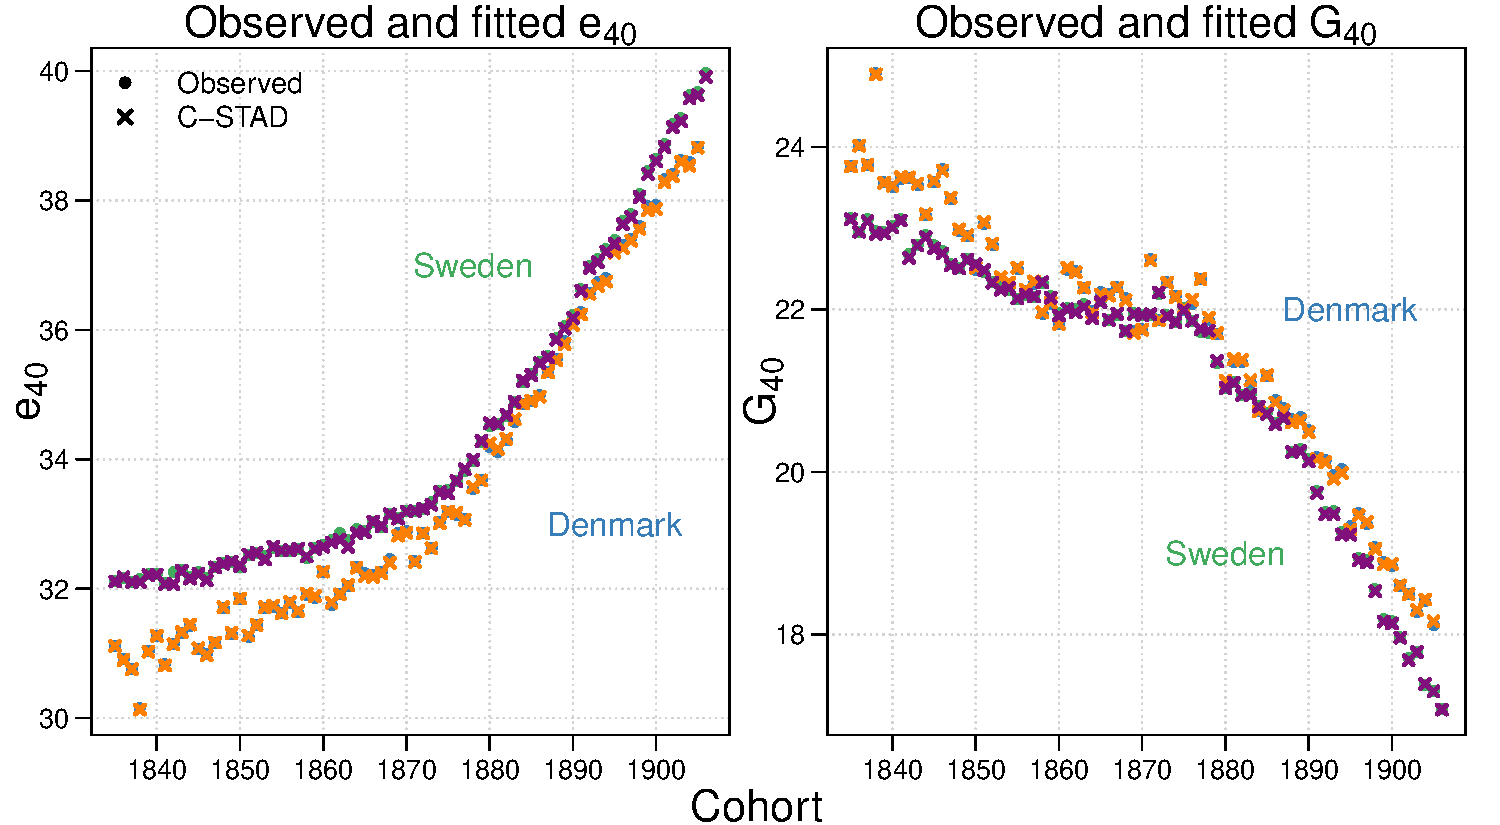
\includegraphics[scale=0.57]{./Figures/F5.pdf} 
		\caption{Observed and C-STAD estimated remaining life expectancies at age 40 ($e_{40}$, left panel) and Gini coefficient at age 40 ($G_{40}$, right panel) for adult females in Sweden and Denmark for the fully observed cohorts 1835--$\breve{c}$ (where $\breve{c}$ is 1906 for Sweden and 1905 for Denmark).\\ \small \textit{Source}: Authors' elaborations on data from the \cite{HMD}.\label{Fig:CSTADfitE40G40}}    
	\end{center}
\end{figure}

Figure \ref{Fig:CSTADforeE40G40} shows the observed (cohorts $\bm{c}_1$) and completed ($\bm{c}_2$ and $\bm{c}_3$) $e_{40}$ and $G_{40}$ computed with the C-STAD (with 80\% pointwise confidence intervals) and 2D $P$-spline model for the two population analysed. Despite sharing similar country trends in the fully observed cohorts $\bm{c}_1$, it is interesting to observe the different mortality developments in the partially observed cohorts $\bm{c}_2$: while Swedish adult females show continuous improvements in longevity and lifespan equality, Danish ones display a stagnation of $e_{40}$ and an increase in lifespan inequality. The trends of the mortality measures for the partially observed cohorts are similar across the models, with the exception of Danish $e_{40}$: the increase of the 2D $P$-spline forecast $e_{40}$ is much faster then for the C-STAD model, resulting in a crossover between the two populations. Moreover, it is interesting to observe that the C-STAD confidence intervals are rather narrow for both countries in $\bm{c}_2$ (as the great majority of data is observed for these cohorts), while they increase in the cohorts $\bm{c}_3$ proportional to the amount of missing data. Note that $\tilde{c}$ is 1925 and 1927 for Sweden and Denmark, respectively.  

\begin{figure}[t]
	\begin{center}
		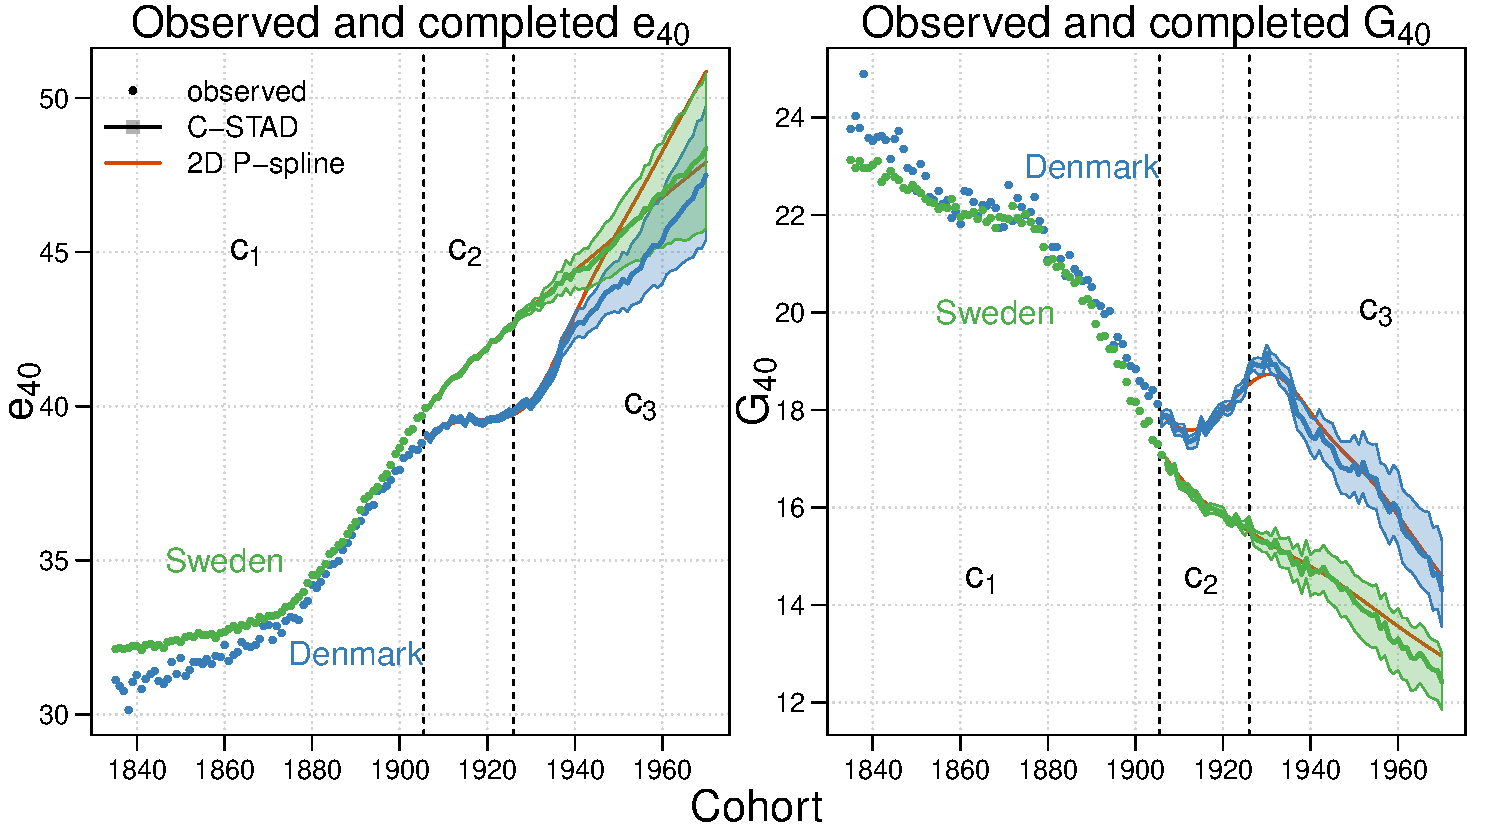
\includegraphics[scale=0.57]{./Figures/F6.pdf} 
		\caption{Observed (cohorts $\bm{c}_1$) and completed ($\bm{c}_2$ and $\bm{c}_3$) remaining life expectancies at age 40 ($e_{40}$, left panel) and Gini coefficient at age 40 ($G_{40}$, right panel) for the C-STAD (with 80\% confidence intervals) and 2D $P$-spline models for adult females in Sweden and Denmark for the cohorts 1835--1970.\\ \small \textit{Source}: Authors' elaborations on data from the \cite{HMD}.\label{Fig:CSTADforeE40G40}}    
	\end{center}
\end{figure}

The age-specific mortality rates analysis shown in Figure \ref{Fig:CSTADforeMx} offers additional insights into cohort mortality developments for the two populations. In the top panels, observed, fitted and forecast mortality rates over cohorts are shown for some selected ages. In addition to the goodness-of-fit of the C-STAD model, the graphs highlight diverse age-specific developments in the two countries: for example, mortality at ages 40 and 60 for Danish cohorts born at the beginning of the twentieth century did not improve, resulting in the atypical trends of the summary measures shown in Figure \ref{Fig:CSTADforeE40G40} (stagnation of $e_{40}$ and increase of $G_{40}$). In the bottom panels, mortality rates over all ages are shown for some selected cohorts. This second perspective shows how the shape of the mortality curve, appropriately captured by the C-STAD model, changed over time: for example, mortality at young adult ages was still relatively high in both countries for the 1835 cohort, with the curve being rather flat in the age range 40--50. The subsequent mortality decline at all ages, mainly attributable to improvements in sanitary environment, public hygiene and nutrition \citep{mckeown1976modern}, clearly emerges from Figure \ref{Fig:CSTADforeMx}. An additional interesting observation is that the confidence intervals of the C-STAD widen as expected: for example, variability increases with age for the completed cohorts, as fewer age-specific data have been observed at higher ages. Finally, Figure \ref{Fig:CSTADforeDx} shows the observed and C-STAD age-at-death distributions for the three cohorts analysed in the previous panels. 

\begin{figure}[h!]
	\begin{center}
		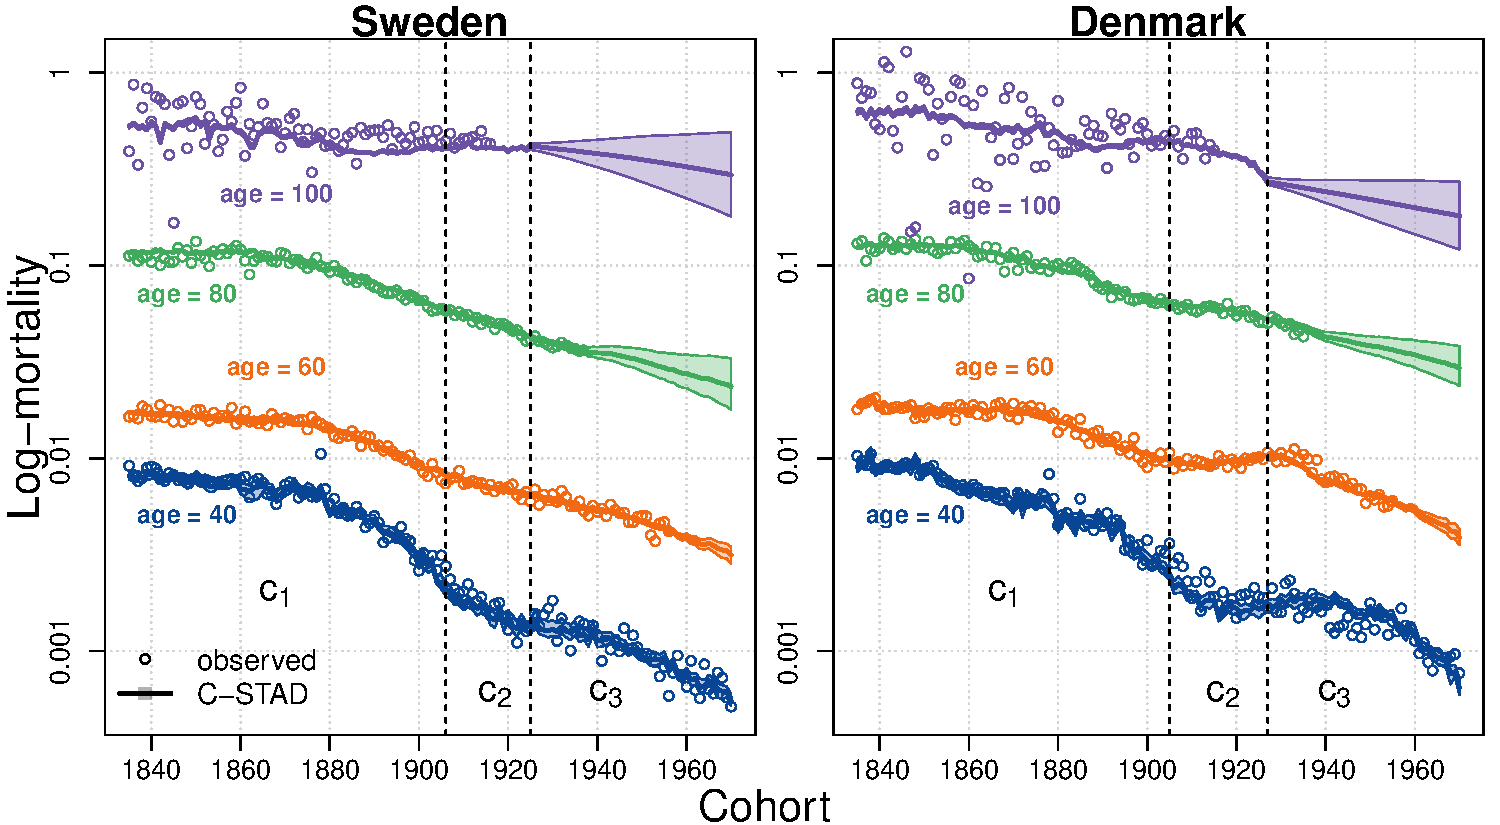
\includegraphics[scale=0.57]{./Figures/F7a.pdf} 
		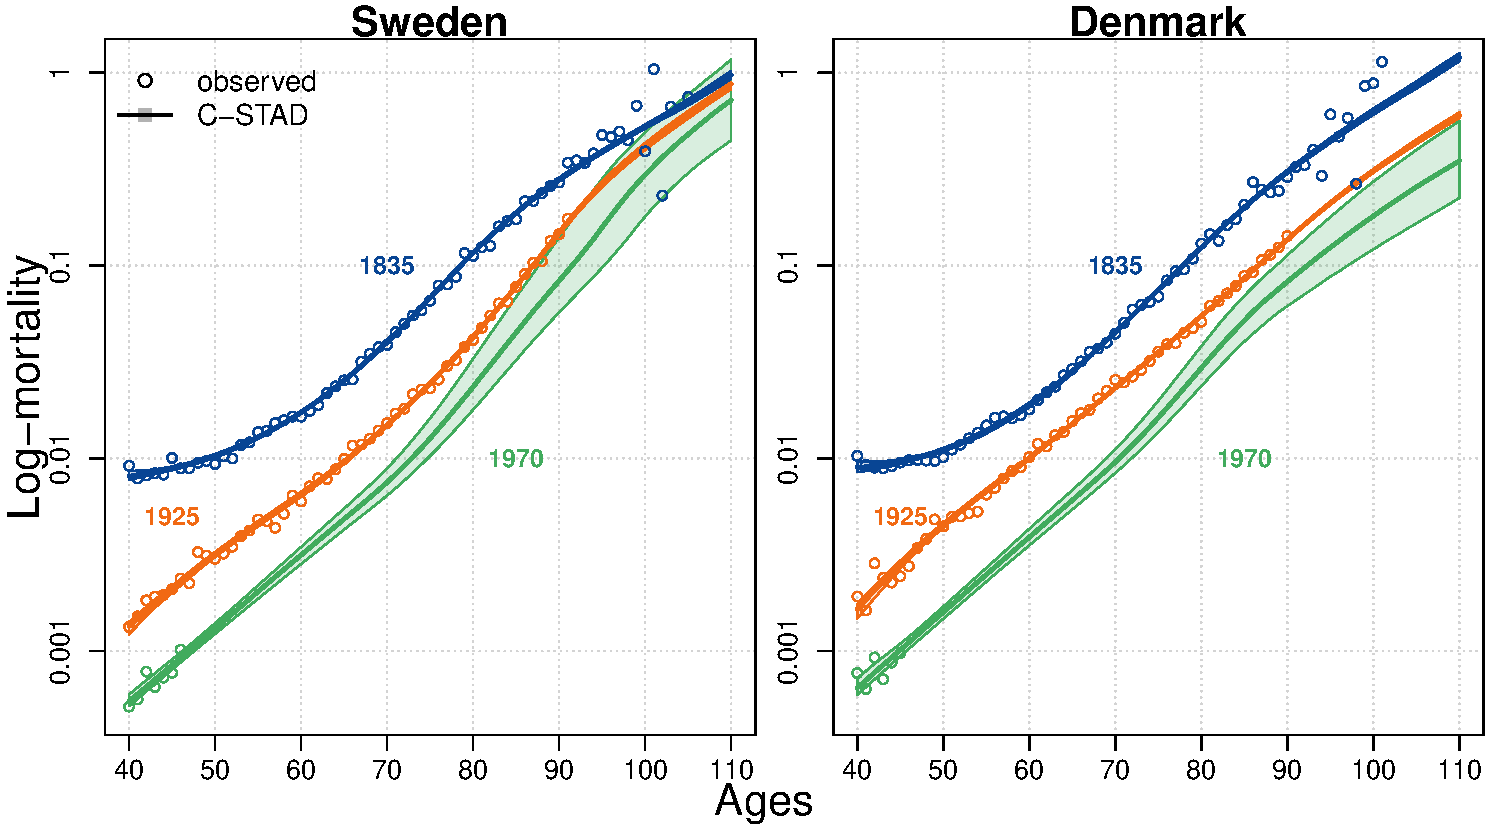
\includegraphics[scale=0.57]{./Figures/F7b.pdf} 
		\caption{Observed, fitted and forecast age-specific mortality rates for selected ages (top panels) and for selected cohorts (bottom panels) with 80\% confidence intervals for females in Sweden and Denmark aged 40--110+ for the cohorts 1835--1970.\\ \small \textit{Source}: Authors' elaborations on data from the \cite{HMD}.\label{Fig:CSTADforeMx}}    
	\end{center}
\end{figure}

\begin{figure}[h!]
	\begin{center}
		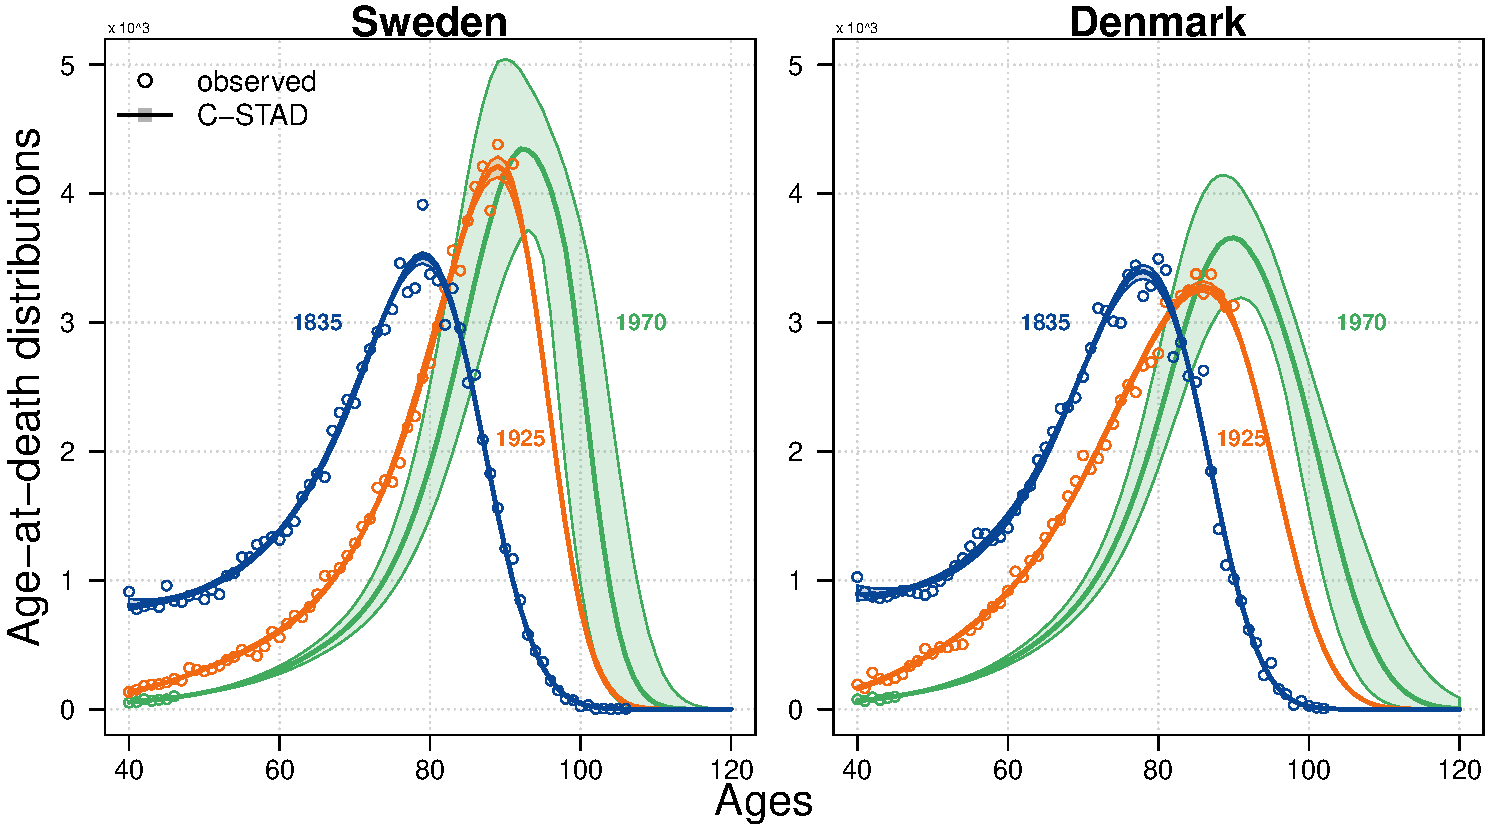
\includegraphics[scale=0.57]{./Figures/F8.pdf}  
		\caption{Observed, fitted and forecast age-at-death distributions for selected cohorts (bottom panels) with 80\% confidence intervals for females in Sweden and Denmark aged 40--110+.\\ \small \textit{Source}: Authors' elaborations on data from the \cite{HMD}.\label{Fig:CSTADforeDx}}    
	\end{center}
\end{figure}

\section{Discussion} 
\label{Sec:Discussion}
Mortality forecasting has drawn considerable interest in recent decades among academics and financial sector practitioners due to the increasing challenges posed by population ageing. Advances in the field have been made almost exclusively on period mortality, as the most recent and innovative techniques are based on modelling and forecasting different functions of period life tables \cite[see, for example,][]{lee1992modeling,cairns2006two,raftery2013bayesian}. When considered, cohort effects in mortality modelling and forecasting are typically analysed within an age-period perspective \citep{renshaw2006cohort,cairns2009quantitative,plat2009stochastic,dokumentov2018bivariate}.  
 
In this article, we take an alternative perspective and introduce a new methodology to model and forecast mortality from cohort data. An important advantage of cohort forecasts is that they allow one to complete the mortality experience of non-extinct cohorts, thus enabling the derivation of their mortality developments. Our approach focuses on cohort age-at-death distributions: specifically, we propose a warping transformation of the age-axis of a standard distribution to describe and forecast adult mortality developments across cohorts. Since we focus on the cohort perspective, we denote our methodology \emph{Cohort Segmented Transformation Age-at-death Distributions} (C-STAD) model. Warping transformations and skewing procedures have already been fruitfully employed to model distributional changes \cite[see, e.g.,][]{fernandez1998bayesian,camarda2008warped}. 

Our methodology is inspired by the Segmented Transformation Age-at-death Distributions (STAD) model recently proposed by \cite{basellini2019modelling} to forecast adult age-at-death distributions. In addition to shifting the focus from period to cohort mortality, our methodology extends the STAD to a cubic transformation before the modal age at death. The additional parameters $c_L$ and $d_L$ are necessary to adequately describe cohort mortality developments at young adult ages. A possible explanation for this is related to the significant improvements in mortality, especially at younger adult ages, across the cohorts that we analyse (cf.~Fig.~\ref{Fig:CSTADforeMx}). Non-linear transformation functions above the mode were tested, but they did not provide a better fit compared to a linear transformation function. 

Only a handful of models have been proposed to directly forecast cohort mortality so far \citep{chiou2009modeling,zanotto2017reconstruction,rizzi2019forecasting}. One of the main reasons for the limited efforts in this direction is the heavy data demands that such models require. However, this problem is reduced when only adult mortality is considered \citep{booth2006demographic}. As such, the issue does not affect us to a great extent, as our interest in this article is restricted to adult mortality only. 

We have shown the results of fitting and forecasting cohort mortality with the C-STAD model for Swedish and Danish adult females aged 40--110 for the cohorts 1835--1970. Our methodology is accurate from a point forecast perspective: for each population, we performed six out-of-sample validation exercises of different forecast horizons. The resulting point forecast errors are generally small, even for the longer forecast horizons. Additionally, the C-STAD forecasts are consistently more precise than those of the 2D $P$-spline model of \cite{currie2004smoothing}, which has already been used to directly forecast cohort mortality \citep{cmi2007stochastic}. 

Furthermore, both age-cohort approaches (the C-STAD and 2D $P$-spline) to forecast cohort mortality perform significantly better than the standard approach of extracting cohort patterns from the diagonals of a projected \cite{lee1992modeling} age-period surface. More generally, age-cohort models are more efficient and parsimonious: looking at Figure~\ref{Fig:Lexis}, the objective of a cohort forecast is to project the green area, which is directly obtained by age-cohort approaches. Conversely, age-period models would also need to forecast all data below the green area as a preliminary step, and then extract the cohort mortality of interest.

Our results allow us to derive age-specific and summary measures of mortality, such as remaining life expectancy and the Gini coefficient at age 40 ($e_{40}$ and $G_{40}$), for all cohorts of the population analysed. Although following similar trends to the 2D $P$-spline model, C-STAD estimates of $e_{40}$ seem to be more coherent when considered together, lacking the rapid increase and cross-over of Danish forecasts displayed by the 2D model. With respect to Danish forecasts, it is interesting to observe a stagnation of $e_{40}$ and an increase of $G_{40}$ for the cohorts 1910--1930. Such results are consistent with other findings in the literature \cite[see, e.g., Fig.~4 in][]{jacobsen2002long}, which have been attributed to the smoking behaviour of Danish women \citep{jacobsen2006causes,lindahl2016did}. 

Since \cite{thiele1871mathematical}, actuaries and demographers have decomposed the age-pattern of mortality into three independent components that mainly operate at childhood, middle and old ages, respectively. Let us denote the three components Childhood, Early-Adulthood and Senescence. Our proposed methodology is specifically designed to model and forecast the Senescent component of mortality. As such, applying the C-STAD from age 40 produces satisfactory results for the female populations analysed in this article because the Childhood and Early-Adulthood components are negligible with respect to the Senescent one in the age range that we study. 
	
Although theoretically and practically possible, we do not recommend applying the model to a (much) wider age range. This would result in a reduction of goodness-of-fit and forecast accuracy, because the C-STAD cannot capture and disentangle the combination of different components at younger ages. A more suitable approach for modelling and forecasting the entire age range would be to decompose and model the mortality pattern by specialized versions of the C-STAD on the component-specific distributions. See \cite{basellini2020three} for an example of this procedure from the age-period perspective.

To conclude, the C-STAD model offers great prospects for mortality forecasting from the cohort perspective. Public and private institutions would benefit from employing our model, as it provides a direct approach to complete the mortality experience  of non-extinct cohorts. The \texttt{R} code provided with this article allows a fast and freely available opportunity for this purpose. 

%\bigskip

\section*{Acknowledgements} 
\label{Sec:Acknowledgements}
The authors would like to thank Mar\'{i}lia Nepomuceno, Roland Rau, Jim Oeppen and an anonymous reviewer for providing useful comments and discussions on this paper. 


\newpage

% BIBLIOGRAPHY: 
\bibliographystyle{apalike}
%\small
\bibliography{Biblio_CSTAD} 

%\newpage
%\bigskip
\appendix
\counterwithin{figure}{section}
\counterwithin{table}{section}
%\normalsize

\section{Deviance residuals and bootstrap death counts}
\label{Appendix:ResidualDeath}     
Model residuals are routinely analysed to explore the goodness-of-fit of a model as well as the adequacy of assumptions about error terms. Within a GLM setting (such as the Poisson considered here), deviance residuals are often used to measure discrepancy between fitted and actual data. For the Poisson distribution they are given by: 
\begin{equation}\label{Eq:DevRes}
r_{\mathrm{D}}= \mathrm{sign} (d_{x,c}-\hat{d}_{x,c}) \, \sqrt{2} \, 
\left[d_{x,c} \ln \left(\frac{d_{x,c}}{\hat{d}_{x,c}}\right) - 
\left(d_{x,c}-\hat{d}_{x,c}\right)
\right]^{1/2}
\end{equation}
where $d_{x,c}$ and $\hat{d}_{x,c}$ denote the observed and fitted death counts at age $x$ and for cohort $c$, respectively \citep{mccullagh1989glm}. 

Deviance residuals can be further employed to take into account the uncertainty related to the estimation of model parameters as suggested by \cite{koissi2006evaluating}. Specifically, bootstrap death counts can be computed by resampling deviance residuals with replacement and mapping them to corresponding death counts. We refer the interested reader to \cite{renshaw2008simulation} for details of the inverse formulas, which are based on the seminal work of \cite{efron1994introduction}.  

\section{Section \ref{Sec:Results}: additional results}
\label{Appendix:AdditResults}     

In this appendix, we present additional results related to Section \ref{Sec:Results}. 

First, Figure \ref{Fig:Alignment} provides an illustration of the landmark registration procedure that we employ to compute the standard from the aligned distributions. The left panel shows the observed smooth distributions derived from the 2D $P$-spline model; in the right panel, the same distributions have been aligned to a common modal age at death, corresponding to the mode of the first cohort (1835). The standard is computed as the mean of the aligned distributions.

\begin{figure}[!ht]
	\begin{center}
		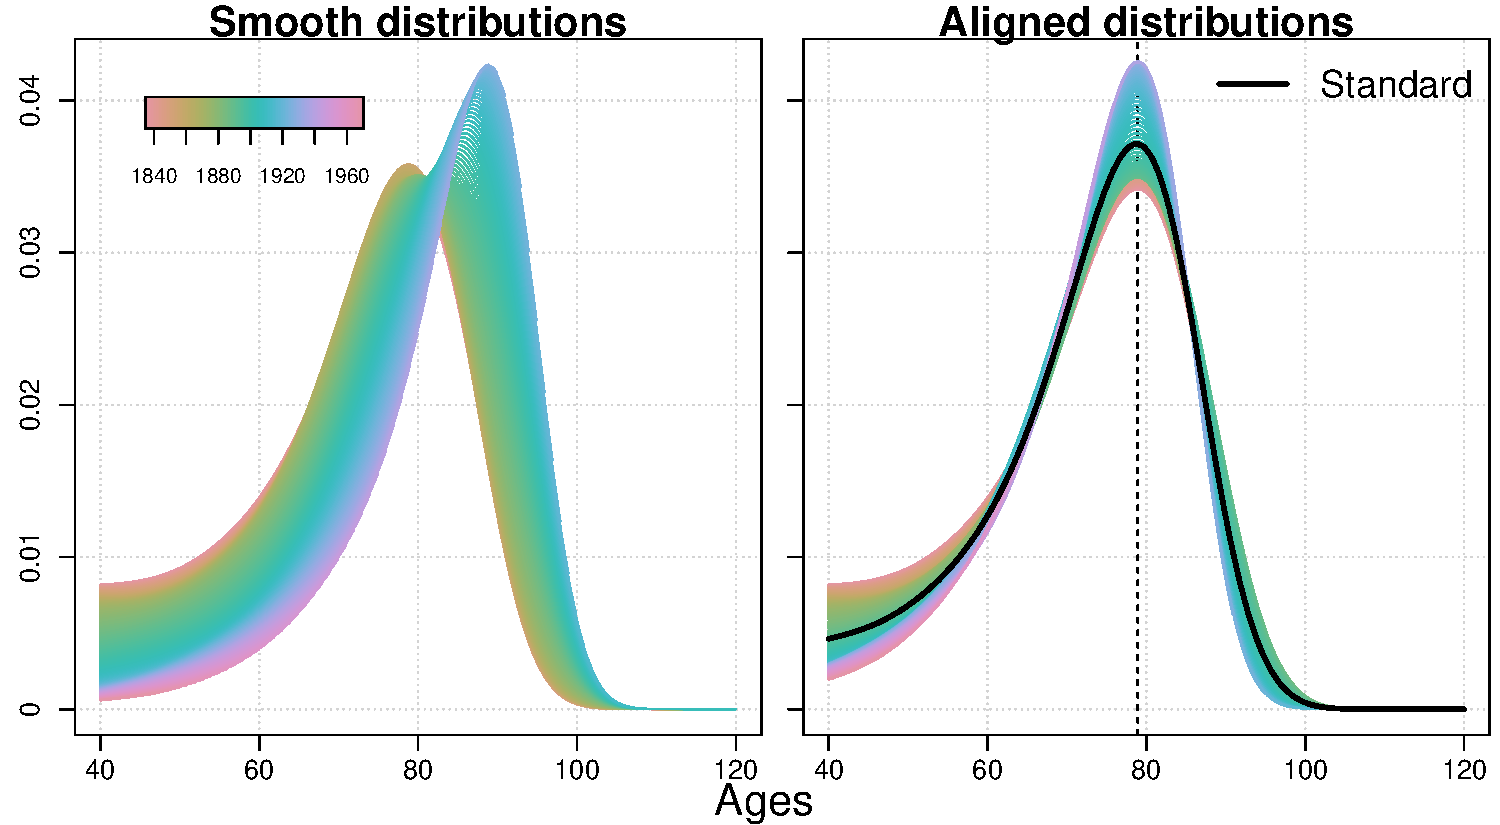
\includegraphics[scale=0.55]{./Figures/FA0.pdf}
		\caption{Observed smooth (left panel) and aligned distributions for Swedish females aged 40--110+ for cohorts 1835--1970. The standard distribution (black line) is computed as the mean of the aligned distributions. \\ \small \textit{Source}: Authors' elaborations on data from the \cite{HMD}.}\label{Fig:Alignment}	
	\end{center}
\end{figure}

Next, we report the out-of-sample results of Subsection \ref{Subsec:Out-of-sample} derived from employing two different prediction accuracy measures. In addition to the root mean square error, we computed the mean absolute error (MAE) and the mean absolute percentage error (MAPE):
%
\begin{equation}\label{Eq:MAE}
\mathrm{MAE} = \frac{1}{h} \sum_{c=1}^{h} \left| \hat{y}_c - y_c \right|  \, , \notag 
\end{equation} 
%
\begin{equation}\label{Eq:MAPE}
\mathrm{MAPE}= \frac{100}{h}  \sum_{c=1}^{h} \left| \frac{\hat{y}_c - y_c}{y_c}  \right| \, , \notag
\end{equation} 
%
where $h$ is the forecasting horizon, and $\hat{y}_c$ and $y_c$ are the forecast and observed out-of-sample values of either $e_{40}$ or $G_{40}$. 

Tables \ref{Table:MAE} and \ref{Table:MAPE} show the out-of-sample results obtained using the MAE and the MAPE, respectively. The results are very similar to those obtained with the RMSE shown in Table \ref{Table:RMSE}: the C-STAD forecasts are accurate in completing the mortality experience of partially observed cohorts, with forecasts errors generally low and smaller than the 2D $P$-spline model. Moreover, both age-cohort models significantly outperform the standard LC age-period based approach, and they are more accurate than the APC model based on the age-period perspective.

Finally, we provide additional results with regard to Subsection \ref{Subsec:ForecastC-STAD}. Figure \ref{Fig:CSTADparams} shows the fitted and forecast C-STAD parameters with 80\% confidence intervals for Swedish and Danish adult females for cohorts 1835--1970.

We performed diagnostic checks on the fitted C-STAD model for the two populations analysed in this paper by using Eq.~\eqref{Eq:DevRes}. Poisson deviance residuals for the two populations are shown in Figure \ref{Fig:CSTADresid}. No clear patterns emerge from this graphical analysis, with the exception of the years corresponding to the Spanish' flu and World War II.


\begin{landscape}  
% TABLE MAE: 10, 20, 30 YEARS
\begin{table}[t]
	\small
	\centering
	\begin{tabular}{cccccccc|cccc}
		\toprule
		& & & &   \multicolumn{4}{c|}{\textbf{Sweden}}    & \multicolumn{4}{c}{\textbf{Denmark}} \\
		
		\cmidrule{5-12}	
		
		\thead{Fitting \\ cohorts}  & \thead{Forecast \\ cohorts} & Horizon &  Measure  &  C-STAD   & \thead{2D \\ $P$-spline} & \thead{LC \\ (period)} & \thead{APC \\ (period)} &  C-STAD   & \thead{2D \\ $P$-spline}  & \thead{LC \\ (period)} &  \thead{APC \\ (period)}  \\ 
		\midrule	
		%%%% FIRST EXERCISE	
		\rowcolor{my-white} 
		\multicolumn{1}{c}{\cellcolor{my-white}}   &
		\multicolumn{1}{c}{\cellcolor{my-white}}   & \multicolumn{1}{c}{\cellcolor{my-white}}               & \multicolumn{1}{c|}{\cellcolor{my-white}$e_{40}$} & 0.08  & \textbf{0.06} & 0.20 & 0.11 &  0.07 &  0.07 & 0.37  & \textbf{0.05}   \\
		\rowcolor{my-white} 
		\multicolumn{1}{c}{\multirow{-2}{*}{\cellcolor{my-white}1835--1895}}  &  \multicolumn{1}{c}{\multirow{-2}{*}{\cellcolor{my-white}1896--1905}}  & 
		\multicolumn{1}{c}{\multirow{-2}{*}{\cellcolor{my-white}10y}}& \multicolumn{1}{c|}{\cellcolor{my-white}$G_{40}$} & \textbf{0.07} & 0.08  & 0.28 & 0.21 & \textbf{0.06} &  0.07 & 0.34 & 0.08 \\
		
		%%%% SECOND EXERCISE	
		\hhline{|------------|}
		\rowcolor{my-grey} 
		\multicolumn{1}{c}{\cellcolor{my-grey}}  & \multicolumn{1}{c}{\cellcolor{my-grey}}             &
		\multicolumn{1}{c}{\cellcolor{my-grey}}  & \multicolumn{1}{c|}{\cellcolor{my-grey}$e_{40}$} & \textbf{0.07} &  0.07 & 0.22 & 0.09 & \textbf{0.06} & 0.07 & 0.35 & 0.06 \\
		\rowcolor{my-grey}       \multicolumn{1}{c}{\multirow{-2}{*}{\cellcolor{my-grey}1835--1890}} &      \multicolumn{1}{c}{\multirow{-2}{*}{\cellcolor{my-grey}1891--1905}}               &
		\multicolumn{1}{c}{\multirow{-2}{*}{\cellcolor{my-grey}15y}}               & \multicolumn{1}{c|}{\cellcolor{my-grey}$G_{40}$} & \textbf{0.07} &  0.08 & 0.35 & 0.20 & \textbf{0.06} & 0.09  & 0.38 & 0.15 \\ 
		
		%%%% THIRD EXERCISE
		\hhline{|------------|}
		\rowcolor{my-white} 
		\multicolumn{1}{c}{\cellcolor{my-white}}   &
		\multicolumn{1}{c}{\cellcolor{my-white}}   &    \multicolumn{1}{c}{\cellcolor{my-white}}                & \multicolumn{1}{c|}{\cellcolor{my-white}$e_{40}$} &  \textbf{0.05} & 0.07 & 0.29 & 0.08 & \textbf{0.06} & 0.07 & 0.38 & 0.07 \\
		\rowcolor{my-white}            
		\multicolumn{1}{c}{\multirow{-2}{*}{\cellcolor{my-white}1835--1885}}           &
		\multicolumn{1}{c}{\multirow{-2}{*}{\cellcolor{my-white}1886--1905}}               &
		\multicolumn{1}{c}{\multirow{-2}{*}{\cellcolor{my-white}20y}}               & \multicolumn{1}{c|}{\cellcolor{my-white}$G_{40}$} & \textbf{0.06} & 0.09 & 0.45 & 0.24 & \textbf{0.05} & 0.09 & 0.39 & 0.19  \\
		
		%%%% FOURTH EXERCISE	
		\hhline{|------------|}
		\rowcolor{my-grey} 
		\multicolumn{1}{c}{\cellcolor{my-grey}}   &
		\multicolumn{1}{c}{\cellcolor{my-grey}}   & \multicolumn{1}{c}{\cellcolor{my-grey}}               & \multicolumn{1}{c|}{\cellcolor{my-grey}$e_{40}$} & \textbf{0.03} & 0.06 & 0.37 & 0.10 & \textbf{0.03} &  0.07 & 0.42  & 0.11  \\
		\rowcolor{my-grey} 
		\multicolumn{1}{c}{\multirow{-2}{*}{\cellcolor{my-grey}1835--1880}}                 &  \multicolumn{1}{c}{\multirow{-2}{*}{\cellcolor{my-grey}1881--1905}}  & 
		\multicolumn{1}{c}{\multirow{-2}{*}{\cellcolor{my-grey}25y}}  & \multicolumn{1}{c|}{\cellcolor{my-grey}$G_{40}$} & \textbf{0.07} & 0.08 & 0.52 & 0.27 & \textbf{0.08} & 0.10  & 0.39  & 0.19  \\
		
		%%%% FIFTH EXERCISE
		\hhline{|------------|}
		\rowcolor{my-white} 
		\multicolumn{1}{c}{\cellcolor{my-white}}             &
		\multicolumn{1}{c}{\cellcolor{my-white}}             & \multicolumn{1}{c}{\cellcolor{my-white}}             & \multicolumn{1}{c|}{\cellcolor{my-white}$e_{40}$} &   \textbf{0.04} & 0.07 & 0.41 & 0.13 &  \textbf{0.02} &  0.08 & 0.46 & 0.14 \\
		\rowcolor{my-white} 
		\multicolumn{1}{c}{\multirow{-2}{*}{\cellcolor{my-white}1835--1875}} &      \multicolumn{1}{c}{\multirow{-2}{*}{\cellcolor{my-white}1876--1905}}               &
		\multicolumn{1}{c}{\multirow{-2}{*}{\cellcolor{my-white}30y}}               & \multicolumn{1}{c|}{\cellcolor{my-white}$G_{40}$} & \textbf{0.08} &  0.12 & 0.55 & 0.31 & \textbf{0.07} & 0.13   & 0.44  & 0.22  \\
		
		%%%% SIXTH EXERCISE
		\hhline{|------------|}
		\rowcolor{my-grey} 
		\multicolumn{1}{c}{\cellcolor{my-grey}}   &   
		\multicolumn{1}{c}{\cellcolor{my-grey}}   &  \multicolumn{1}{c}{\cellcolor{my-grey}}                & \multicolumn{1}{c|}{\cellcolor{my-grey}$e_{40}$} & 0.09 & \textbf{0.07} & 0.48 & 0.12 & \textbf{0.04} &  0.10 & 0.49 & 0.13 \\
		\rowcolor{my-grey}           
		\multicolumn{1}{c}{\multirow{-2}{*}{\cellcolor{my-grey}1835--1870}}           &
		\multicolumn{1}{c}{\multirow{-2}{*}{\cellcolor{my-grey}1871--1905}}               &
		\multicolumn{1}{c}{\multirow{-2}{*}{\cellcolor{my-grey}35y}}               & \multicolumn{1}{c|}{\cellcolor{my-grey}$G_{40}$} & \textbf{0.03} &  0.10 & 0.52 & 0.33 & \textbf{0.05} & 0.17 & 0.43 & 0.25 \\		
		
		\bottomrule 
		
	\end{tabular}
	\caption{Mean absolute error (MAE) of the C-STAD, 2D $P$-spline, LC (on the age-period perspective) and APC (on the age-period perspective) forecasts of $e_{40}$ and $G_{40}$ for adult females in Sweden and Denmark in six out-of-sample validation exercises: forecast horizon of 10, 15, 20, 25, 30 and 35 years. Lower values of the MAE (in bold, assessed using all available decimals) correspond to greater forecast accuracy.\\ \small \textit{Source}: Authors' elaborations on data from the \cite{HMD}.}\label{Table:MAE}
\end{table}
%\end{landscape}

%\begin{landscape}
% TABLE MAPE: 10, 20, 30 YEARS
\begin{table}[t]
	\small
	\centering
	\begin{tabular}{cccccccc|cccc}
		\toprule
		& & & &   \multicolumn{4}{c|}{\textbf{Sweden}}    & \multicolumn{4}{c}{\textbf{Denmark}} \\
		
		\cmidrule{5-12}	
		
		\thead{Fitting \\ cohorts}  & \thead{Forecast \\ cohorts} & Horizon &  Measure  &  C-STAD   & \thead{2D \\ $P$-spline} & \thead{LC \\ (period)} & \thead{APC \\ (period)} &  C-STAD   & \thead{2D \\ $P$-spline}  & \thead{LC \\ (period)} &  \thead{APC \\ (period)}  \\ 
		\midrule	
		%%%% FIRST EXERCISE	
		\rowcolor{my-white} 
		\multicolumn{1}{c}{\cellcolor{my-white}}   &
		\multicolumn{1}{c}{\cellcolor{my-white}}   & \multicolumn{1}{c}{\cellcolor{my-white}}               & \multicolumn{1}{c|}{\cellcolor{my-white}$e_{40}$} & 0.20\%  & \textbf{0.16\%} & 0.51\% & 0.28\% &  0.19\% & 0.19\% & 0.96\% & \textbf{0.12\%} \\
		\rowcolor{my-white} 
		\multicolumn{1}{c}{\multirow{-2}{*}{\cellcolor{my-white}1835--1895}}  &  \multicolumn{1}{c}{\multirow{-2}{*}{\cellcolor{my-white}1896--1905}}  & 
		\multicolumn{1}{c}{\multirow{-2}{*}{\cellcolor{my-white}10y}}& \multicolumn{1}{c|}{\cellcolor{my-white}$G_{40}$} & \textbf{0.42\%} &   0.45\% & 1.57\% & 1.18\% & \textbf{0.35\%} &  0.36\% & 1.83\% & 0.42\%  \\
		
		%%%% SECOND EXERCISE	
		\hhline{|------------|}
		\rowcolor{my-grey} 
		\multicolumn{1}{c}{\cellcolor{my-grey}}  & \multicolumn{1}{c}{\cellcolor{my-grey}}             &
		\multicolumn{1}{c}{\cellcolor{my-grey}}  & \multicolumn{1}{c|}{\cellcolor{my-grey}$e_{40}$} & \textbf{0.17\%} &   0.19\% & 0.58\% & 0.23\% & \textbf{0.16\%} &  0.19\% & 0.93\% & 0.17\% \\
		\rowcolor{my-grey}       \multicolumn{1}{c}{\multirow{-2}{*}{\cellcolor{my-grey}1835--1890}} &      \multicolumn{1}{c}{\multirow{-2}{*}{\cellcolor{my-grey}1891--1905}}               &
		\multicolumn{1}{c}{\multirow{-2}{*}{\cellcolor{my-grey}15y}}               & \multicolumn{1}{c|}{\cellcolor{my-grey}$G_{40}$} & \textbf{0.36\%} &   0.45\% & 1.93\% & 1.08\% & \textbf{0.30\%} &  0.47\% & 2.04\%  & 0.76\%  \\ 
		
		%%%% THIRD EXERCISE
		\hhline{|------------|}
		\rowcolor{my-white} 
		\multicolumn{1}{c}{\cellcolor{my-white}}   &
		\multicolumn{1}{c}{\cellcolor{my-white}}   &    \multicolumn{1}{c}{\cellcolor{my-white}}                & \multicolumn{1}{c|}{\cellcolor{my-white}$e_{40}$} &  \textbf{0.13\%} &   0.19\% & 0.77\% & 0.22\% & \textbf{0.15\%} &  0.18\% & 1.02\% & 0.19\% \\
		\rowcolor{my-white}            
		\multicolumn{1}{c}{\multirow{-2}{*}{\cellcolor{my-white}1835--1885}}           &
		\multicolumn{1}{c}{\multirow{-2}{*}{\cellcolor{my-white}1886--1905}}               &
		\multicolumn{1}{c}{\multirow{-2}{*}{\cellcolor{my-white}20y}}               & \multicolumn{1}{c|}{\cellcolor{my-white}$G_{40}$} & \textbf{0.34\%} &  0.46\% & 2.40\% & 1.26\% & \textbf{0.27\%} &  0.44\% & 2.02\% & 0.96\% \\
		
		%%%% FOURTH EXERCISE	
		\hhline{|------------|}
		\rowcolor{my-grey} 
		\multicolumn{1}{c}{\cellcolor{my-grey}}   &
		\multicolumn{1}{c}{\cellcolor{my-grey}}   & \multicolumn{1}{c}{\cellcolor{my-grey}}               & \multicolumn{1}{c|}{\cellcolor{my-grey}$e_{40}$} & \textbf{0.08\%} &   0.17\% & 0.98\% & 0.27\% & \textbf{0.08\%} &  0.18\% & 1.14\%   & 0.30\%  \\
		\rowcolor{my-grey} 
		\multicolumn{1}{c}{\multirow{-2}{*}{\cellcolor{my-grey}1835--1880}}                 &  \multicolumn{1}{c}{\multirow{-2}{*}{\cellcolor{my-grey}1881--1905}}  & 
		\multicolumn{1}{c}{\multirow{-2}{*}{\cellcolor{my-grey}25y}}  & \multicolumn{1}{c|}{\cellcolor{my-grey}$G_{40}$} & \textbf{0.40\%} &  0.44\% & 2.71\% & 1.39\% & \textbf{0.42\%} &  0.51\% & 2.05\%  & 0.96\%    \\
		
		%%%% FIFTH EXERCISE
		\hhline{|------------|}
		\rowcolor{my-white} 
		\multicolumn{1}{c}{\cellcolor{my-white}}             &
		\multicolumn{1}{c}{\cellcolor{my-white}}             & \multicolumn{1}{c}{\cellcolor{my-white}}             & \multicolumn{1}{c|}{\cellcolor{my-white}$e_{40}$} &   \textbf{0.10\%} &   0.20\% & 1.12\% & 0.36\% & \textbf{0.07\%} &  0.23\% & 1.28\% & 0.37\%  \\
		\rowcolor{my-white} 
		\multicolumn{1}{c}{\multirow{-2}{*}{\cellcolor{my-white}1835--1875}} &      \multicolumn{1}{c}{\multirow{-2}{*}{\cellcolor{my-white}1876--1905}}               &
		\multicolumn{1}{c}{\multirow{-2}{*}{\cellcolor{my-white}30y}}               & \multicolumn{1}{c|}{\cellcolor{my-white}$G_{40}$} & \textbf{0.42\%} &  0.59\% & 2.84\% & 1.55\% & \textbf{0.39\%} &  0.63\% & 2.21\%  & 1.10\%     \\
		
		%%%% SIXTH EXERCISE
		\hhline{|------------|}
		\rowcolor{my-grey} 
		\multicolumn{1}{c}{\cellcolor{my-grey}}   &   
		\multicolumn{1}{c}{\cellcolor{my-grey}}   &  \multicolumn{1}{c}{\cellcolor{my-grey}}                & \multicolumn{1}{c|}{\cellcolor{my-grey}$e_{40}$} & 0.22\% &  \textbf{0.19\%} & 1.33\% & 0.34\% & \textbf{0.12\%} &  0.29\% & 1.36\% & 0.36\%  \\
		\rowcolor{my-grey}           
		\multicolumn{1}{c}{\multirow{-2}{*}{\cellcolor{my-grey}1835--1870}}           &
		\multicolumn{1}{c}{\multirow{-2}{*}{\cellcolor{my-grey}1871--1905}}               &
		\multicolumn{1}{c}{\multirow{-2}{*}{\cellcolor{my-grey}35y}}               & \multicolumn{1}{c|}{\cellcolor{my-grey}$G_{40}$} & \textbf{0.14\%} &  0.51\% & 2.62\% & 1.67\% & \textbf{0.23\%} &  0.81\% & 2.09\% & 1.19\%  \\		
		
		\bottomrule 
		
	\end{tabular}
	\caption{Mean absolute percentage error (MAPE) of the C-STAD, 2D $P$-spline, LC (on the age-period perspective) and APC (on the age-period perspective) forecasts of $e_{40}$ and $G_{40}$ for adult females in Sweden and Denmark in six out-of-sample validation exercises: forecast horizon of 10, 15, 20, 25, 30 and 35 years. Lower values of the MAPE (in bold, assessed using all available decimals) correspond to greater forecast accuracy. \small \textit{Source}: Authors' elaborations on data from the \cite{HMD}. }\label{Table:MAPE}
\end{table}
\end{landscape}

\begin{landscape}
	\begin{figure}[h!]
		\begin{center}
			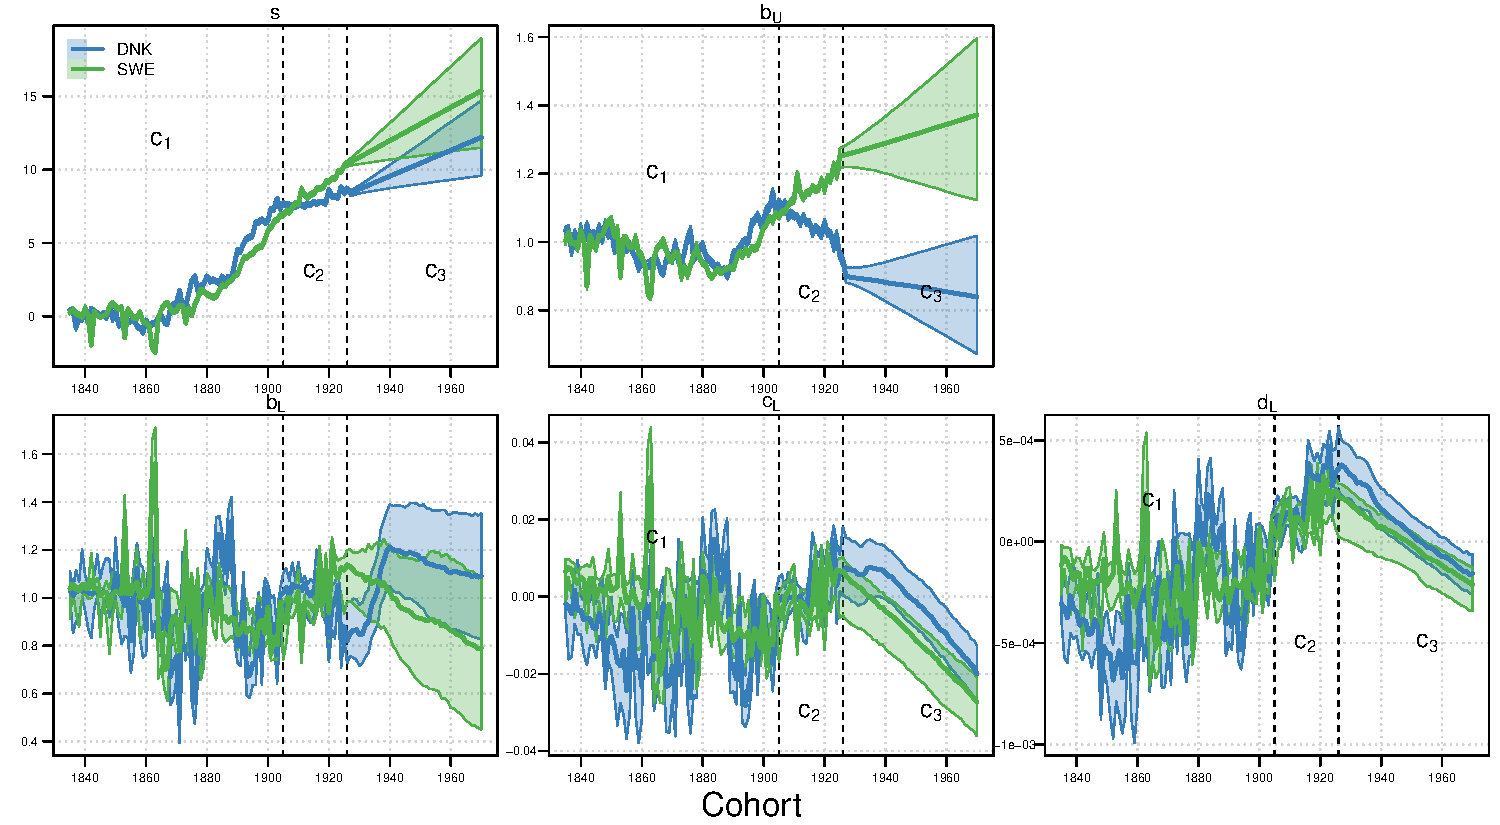
\includegraphics[scale=0.92]{./Figures/FA1.pdf} 
			\caption{Estimated and forecast C-STAD parameters for adult females in Sweden and Denmark for the cohorts 1835--1970. \\ \small \textit{Source}: Authors' elaborations on data from the \cite{HMD}.\label{Fig:CSTADparams}}    
		\end{center}
	\end{figure}
\end{landscape}
 
\begin{landscape}
	\begin{figure}[h!]
		\begin{center}
			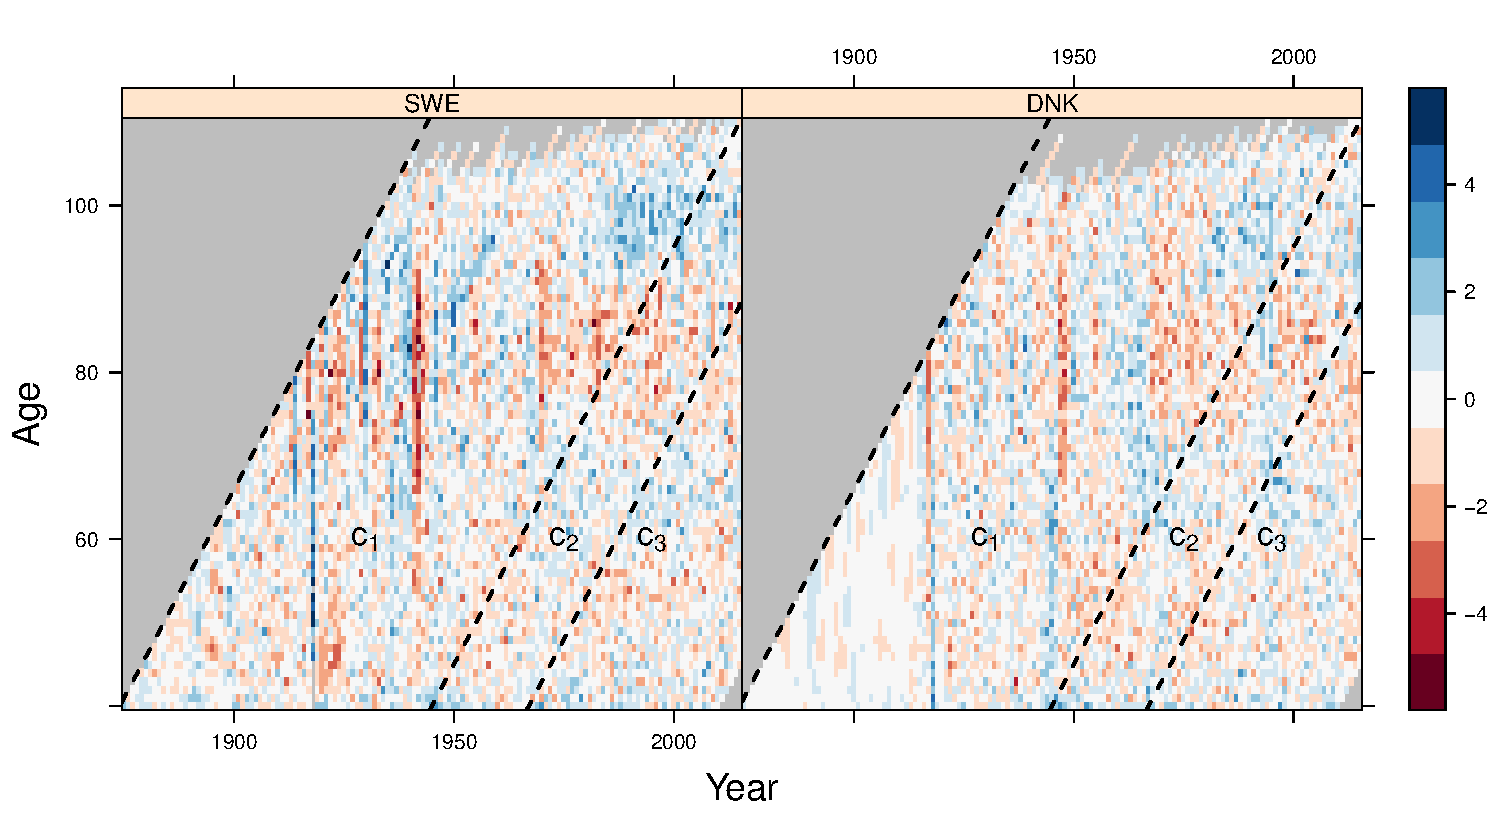
\includegraphics[scale=0.92]{./Figures/FA2.pdf} 
			\caption{Poisson deviance residuals of the C-STAD model for adult females in Sweden and Denmark for the cohorts 1835--1970.\\ \small \textit{Source}: Authors' elaborations on data from the \cite{HMD}.\label{Fig:CSTADresid}}    
		\end{center}
	\end{figure}
\end{landscape}


 
\end{document} 